%\renewcommand{\theequation}{\theenumi}
%\begin{enumerate}[label=\arabic*.,ref=\thesubsection.\theenumi]
%\numberwithin{equation}{enumi}
%
\item A town B is located 36km east and 15 km north of the town A.  How would you find the distance from town A to town B without actually measuring it?
\\
\solution
From theory, we understand that using dot product we can find the angle between the lines 
\begin{enumerate}
	\item 
	\begin{align}\label{eq:solutions/line_plane/74/codes:5}
		\frac{x-2}{2} = \frac{y-1}{5} &= \frac{z+3}{-3}, 
	\end{align}
	\begin{align}\label{eq:solutions/line_plane/74/codes:6}
		\frac{x+2}{-1} = \frac{y-4}{8} &= \frac{z-5}{4} 
	\end{align}


The above symmetric equations \ref{eq:solutions/line_plane/74/codes:5}, \ref{eq:solutions/line_plane/74/codes:6} can be represented in the vector form as 
\begin{align}\label{eq:solutions/line_plane/74/codes7}
	\quad \vec{r_1} &= \myvec{2\\1\\-3} + \lambda_1\myvec{2\\5\\-3}
	\\
	\quad \vec{r_2} &= \myvec{-2\\4\\5} + \lambda_2\myvec{-1\\8\\4}
\end{align}

As we have to find the angle between the vectors, we will only be taking the direction vectors into consideration. The direction vectors are $\vec{u}$ = $\myvec{2\\5\\-3}$ and $\vec{v}$ = $\myvec{-1\\8\\4}$. We can find the corresponding magnitude values

\begin{align}\label{eq:solutions/line_plane/74/codes9}
	\norm{\vec{u}} =\sqrt{2^{2}+5^{2}+(-3)^{2}} =\sqrt{38}
\end{align}
\begin{align}\label{eq:solutions/line_plane/74/codes10}
	\norm{\vec{v}} =\sqrt{(-1)^{2}+8^{2}+4^{2}} =\sqrt{81}
\end{align}

Using \ref{eq:solutions/line_plane/74/codes4}, \ref{eq:solutions/line_plane/74/codes9}, \ref{eq:solutions/line_plane/74/codes10} we get
\begin{align}
	\theta = \cos ^{-1}\frac{\myvec{2\\5\\-3}^{T}\myvec{-1\\8\\4}}{(\sqrt{38})(\sqrt{81})} 
	\\
	\theta = \cos ^{-1}\frac{26}{55.4797}
	\\
	\theta = \cos ^{-1} (0.4686)
	\\
	\theta = 62.053\degree
\end{align}

Therefore, the angle between the two lines is $62.053\degree$.See Fig. \ref{fig:solutions/line_plane/74/codesline_equation_1}

\begin{figure}
	\centering
	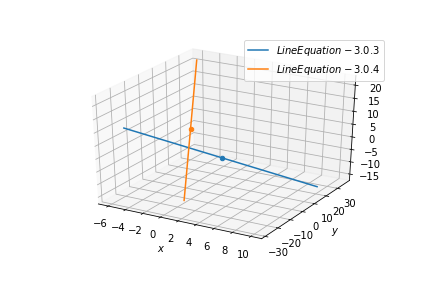
\includegraphics[width=\columnwidth]{./solutions/line_plane/74/codes/figs/Line_interest_1.png}
	\caption{Graph for equations \ref{eq:solutions/line_plane/74/codes7}}
	\label{fig:solutions/line_plane/74/codesline_equation_1}
\end{figure}


	\item 
	\begin{align}\label{eq:solutions/line_plane/74/codes12}
		\frac{x}{2} = \frac{y}{2} &= \frac{z}{1}, 
	\end{align}
	\begin{align}\label{eq:solutions/line_plane/74/codes13}
		\frac{x-5}{4} = \frac{y-2}{1} &= \frac{z-3}{8} 
	\end{align}



The above symmetric equations \ref{eq:solutions/line_plane/74/codes12}, \ref{eq:solutions/line_plane/74/codes13} can be represented in the vector form as 
\begin{align}\label{eq:solutions/line_plane/74/codes14}
	\quad \vec{r_1} &= \myvec{0\\0\\0} + \lambda_1\myvec{2\\2\\1}
	\\
	\quad \vec{r_2} &= \myvec{5\\2\\3} + \lambda_2\myvec{4\\1\\8}
\end{align}

As we have to find the angle between the vectors, we will only be taking the direction vectors into consideration. The direction vectors are $\vec{u}$ = $\myvec{2\\2\\1}$ and $\vec{v}$ = $\myvec{4\\1\\8}$. We can find the corresponding magnitude values

\begin{align}\label{eq:solutions/line_plane/74/codes16}
	\norm{\vec{u}} =\sqrt{2^{2}+2^{2}+1^{2}} =\sqrt{9}
\end{align}
\begin{align}\label{eq:solutions/line_plane/74/codes17}
	\norm{\vec{v}} =\sqrt{4^{2}+1^{2}+8^{2}} =\sqrt{81}
\end{align}

Using \ref{eq:solutions/line_plane/74/codes4}, \ref{eq:solutions/line_plane/74/codes16}, \ref{eq:solutions/line_plane/74/codes17} we get
\begin{align}
	\theta = \cos ^{-1}\frac{\myvec{2\\2\\1}^{T}\myvec{4\\1\\8}}{(\sqrt{9})(\sqrt{81})} 
	\\
	\theta = \cos ^{-1}\frac{18}{27.00}
	\\
	\theta = \cos ^{-1} (0.667)
	\\
	\theta = 48.189\degree
\end{align}

Therefore, the angle between the two lines is $48.189\degree$. See Fig. \ref{fig:solutions/line_plane/74/codesline_equation_2}


\begin{figure}
	\centering
	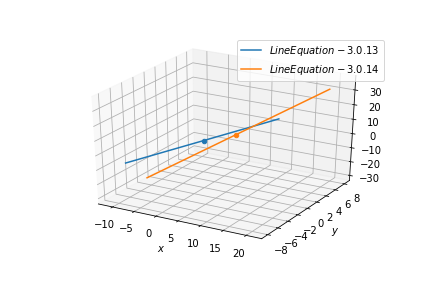
\includegraphics[width=\columnwidth]{./solutions/line_plane/74/codes/figs/Line_interest_2.png}
	\caption{Graph for equations \ref{eq:solutions/line_plane/74/codes14}}
	\label{fig:solutions/line_plane/74/codesline_equation_2}
\end{figure}
\end{enumerate}

    

\item Find the angle between the x-axis and the line joining the points \myvec{3\\–1} and \myvec{4\\–2}.
\solution

	\begin{align}
\frac{ \brak{\vec{A}-\vec{B}}^T\myvec{1 \\ 0}}{\norm{\vec{A}-\vec{B}}\norm{\myvec{1 \\ 0}}} &= \frac{\myvec{-1 &1}^T\myvec{1 \\ 0}}{\norm{\myvec{-1 \\1}}\norm{\myvec{-1 \\1}}}
\\
&= -\frac{1}{\sqrt{2}} = \cos ^{-1}\brak{135\degree}
	\end{align}
Thus, the desired angle is $135\degree$.
	The following python code generates Fig. \ref{fig:3.5.5_qnine}.
	\begin{lstlisting}
	./solutions/5/codes/lines/q9.py
	\end{lstlisting}

	\begin{figure}[!ht]
	\centering
	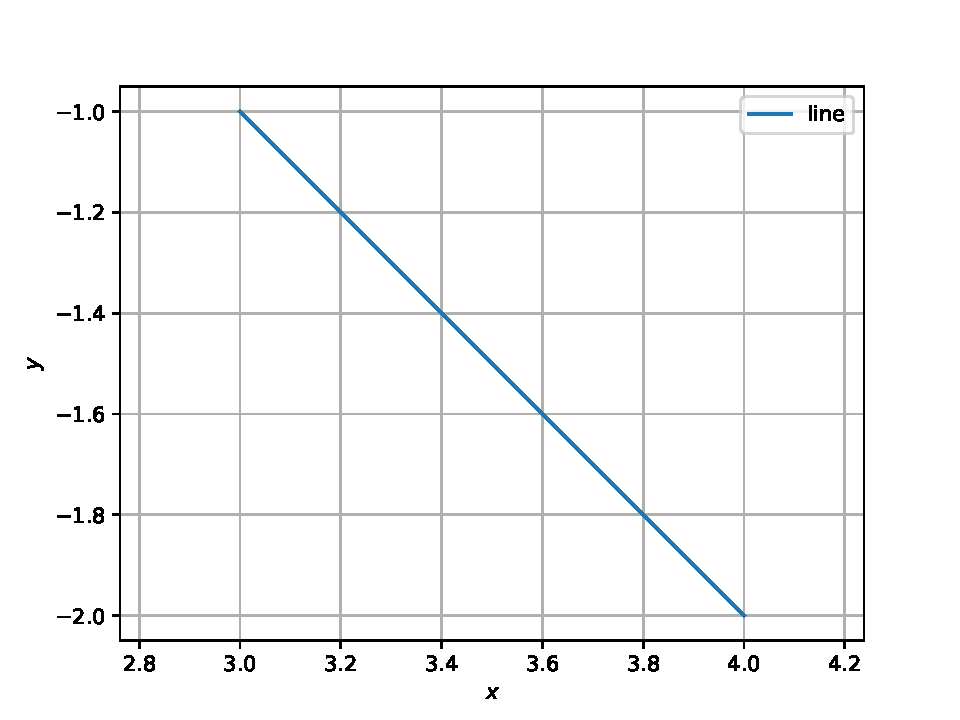
\includegraphics[width=\columnwidth]{./solutions/5/figs/lines/q9.eps}
	\caption{}
	\label{fig:3.5.5_qnine}	
	\end{figure}
	


\item Find the point on the $x$-axis which is equidistant from 
\begin{align}
\myvec{2\\-5}, \myvec{-2\\9},
\end{align}
\solution
From theory, we understand that using dot product we can find the angle between the lines 
\begin{enumerate}
	\item 
	\begin{align}\label{eq:solutions/line_plane/74/codes:5}
		\frac{x-2}{2} = \frac{y-1}{5} &= \frac{z+3}{-3}, 
	\end{align}
	\begin{align}\label{eq:solutions/line_plane/74/codes:6}
		\frac{x+2}{-1} = \frac{y-4}{8} &= \frac{z-5}{4} 
	\end{align}


The above symmetric equations \ref{eq:solutions/line_plane/74/codes:5}, \ref{eq:solutions/line_plane/74/codes:6} can be represented in the vector form as 
\begin{align}\label{eq:solutions/line_plane/74/codes7}
	\quad \vec{r_1} &= \myvec{2\\1\\-3} + \lambda_1\myvec{2\\5\\-3}
	\\
	\quad \vec{r_2} &= \myvec{-2\\4\\5} + \lambda_2\myvec{-1\\8\\4}
\end{align}

As we have to find the angle between the vectors, we will only be taking the direction vectors into consideration. The direction vectors are $\vec{u}$ = $\myvec{2\\5\\-3}$ and $\vec{v}$ = $\myvec{-1\\8\\4}$. We can find the corresponding magnitude values

\begin{align}\label{eq:solutions/line_plane/74/codes9}
	\norm{\vec{u}} =\sqrt{2^{2}+5^{2}+(-3)^{2}} =\sqrt{38}
\end{align}
\begin{align}\label{eq:solutions/line_plane/74/codes10}
	\norm{\vec{v}} =\sqrt{(-1)^{2}+8^{2}+4^{2}} =\sqrt{81}
\end{align}

Using \ref{eq:solutions/line_plane/74/codes4}, \ref{eq:solutions/line_plane/74/codes9}, \ref{eq:solutions/line_plane/74/codes10} we get
\begin{align}
	\theta = \cos ^{-1}\frac{\myvec{2\\5\\-3}^{T}\myvec{-1\\8\\4}}{(\sqrt{38})(\sqrt{81})} 
	\\
	\theta = \cos ^{-1}\frac{26}{55.4797}
	\\
	\theta = \cos ^{-1} (0.4686)
	\\
	\theta = 62.053\degree
\end{align}

Therefore, the angle between the two lines is $62.053\degree$.See Fig. \ref{fig:solutions/line_plane/74/codesline_equation_1}

\begin{figure}
	\centering
	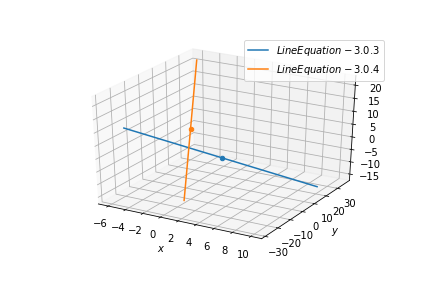
\includegraphics[width=\columnwidth]{./solutions/line_plane/74/codes/figs/Line_interest_1.png}
	\caption{Graph for equations \ref{eq:solutions/line_plane/74/codes7}}
	\label{fig:solutions/line_plane/74/codesline_equation_1}
\end{figure}


	\item 
	\begin{align}\label{eq:solutions/line_plane/74/codes12}
		\frac{x}{2} = \frac{y}{2} &= \frac{z}{1}, 
	\end{align}
	\begin{align}\label{eq:solutions/line_plane/74/codes13}
		\frac{x-5}{4} = \frac{y-2}{1} &= \frac{z-3}{8} 
	\end{align}



The above symmetric equations \ref{eq:solutions/line_plane/74/codes12}, \ref{eq:solutions/line_plane/74/codes13} can be represented in the vector form as 
\begin{align}\label{eq:solutions/line_plane/74/codes14}
	\quad \vec{r_1} &= \myvec{0\\0\\0} + \lambda_1\myvec{2\\2\\1}
	\\
	\quad \vec{r_2} &= \myvec{5\\2\\3} + \lambda_2\myvec{4\\1\\8}
\end{align}

As we have to find the angle between the vectors, we will only be taking the direction vectors into consideration. The direction vectors are $\vec{u}$ = $\myvec{2\\2\\1}$ and $\vec{v}$ = $\myvec{4\\1\\8}$. We can find the corresponding magnitude values

\begin{align}\label{eq:solutions/line_plane/74/codes16}
	\norm{\vec{u}} =\sqrt{2^{2}+2^{2}+1^{2}} =\sqrt{9}
\end{align}
\begin{align}\label{eq:solutions/line_plane/74/codes17}
	\norm{\vec{v}} =\sqrt{4^{2}+1^{2}+8^{2}} =\sqrt{81}
\end{align}

Using \ref{eq:solutions/line_plane/74/codes4}, \ref{eq:solutions/line_plane/74/codes16}, \ref{eq:solutions/line_plane/74/codes17} we get
\begin{align}
	\theta = \cos ^{-1}\frac{\myvec{2\\2\\1}^{T}\myvec{4\\1\\8}}{(\sqrt{9})(\sqrt{81})} 
	\\
	\theta = \cos ^{-1}\frac{18}{27.00}
	\\
	\theta = \cos ^{-1} (0.667)
	\\
	\theta = 48.189\degree
\end{align}

Therefore, the angle between the two lines is $48.189\degree$. See Fig. \ref{fig:solutions/line_plane/74/codesline_equation_2}


\begin{figure}
	\centering
	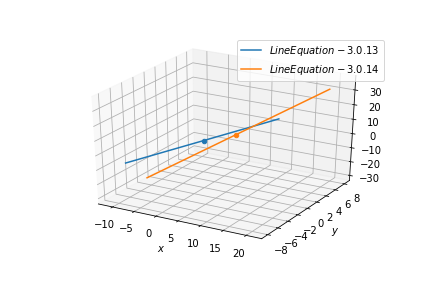
\includegraphics[width=\columnwidth]{./solutions/line_plane/74/codes/figs/Line_interest_2.png}
	\caption{Graph for equations \ref{eq:solutions/line_plane/74/codes14}}
	\label{fig:solutions/line_plane/74/codesline_equation_2}
\end{figure}
\end{enumerate}

    

\item Find the values of $y$ for which the distance between the points 
\begin{align}
\vec{P} = \myvec{2\\-3}, \vec{Q} = \myvec{10\\y}
\end{align}
is 10 units.
\solution
From theory, we understand that using dot product we can find the angle between the lines 
\begin{enumerate}
	\item 
	\begin{align}\label{eq:solutions/line_plane/74/codes:5}
		\frac{x-2}{2} = \frac{y-1}{5} &= \frac{z+3}{-3}, 
	\end{align}
	\begin{align}\label{eq:solutions/line_plane/74/codes:6}
		\frac{x+2}{-1} = \frac{y-4}{8} &= \frac{z-5}{4} 
	\end{align}


The above symmetric equations \ref{eq:solutions/line_plane/74/codes:5}, \ref{eq:solutions/line_plane/74/codes:6} can be represented in the vector form as 
\begin{align}\label{eq:solutions/line_plane/74/codes7}
	\quad \vec{r_1} &= \myvec{2\\1\\-3} + \lambda_1\myvec{2\\5\\-3}
	\\
	\quad \vec{r_2} &= \myvec{-2\\4\\5} + \lambda_2\myvec{-1\\8\\4}
\end{align}

As we have to find the angle between the vectors, we will only be taking the direction vectors into consideration. The direction vectors are $\vec{u}$ = $\myvec{2\\5\\-3}$ and $\vec{v}$ = $\myvec{-1\\8\\4}$. We can find the corresponding magnitude values

\begin{align}\label{eq:solutions/line_plane/74/codes9}
	\norm{\vec{u}} =\sqrt{2^{2}+5^{2}+(-3)^{2}} =\sqrt{38}
\end{align}
\begin{align}\label{eq:solutions/line_plane/74/codes10}
	\norm{\vec{v}} =\sqrt{(-1)^{2}+8^{2}+4^{2}} =\sqrt{81}
\end{align}

Using \ref{eq:solutions/line_plane/74/codes4}, \ref{eq:solutions/line_plane/74/codes9}, \ref{eq:solutions/line_plane/74/codes10} we get
\begin{align}
	\theta = \cos ^{-1}\frac{\myvec{2\\5\\-3}^{T}\myvec{-1\\8\\4}}{(\sqrt{38})(\sqrt{81})} 
	\\
	\theta = \cos ^{-1}\frac{26}{55.4797}
	\\
	\theta = \cos ^{-1} (0.4686)
	\\
	\theta = 62.053\degree
\end{align}

Therefore, the angle between the two lines is $62.053\degree$.See Fig. \ref{fig:solutions/line_plane/74/codesline_equation_1}

\begin{figure}
	\centering
	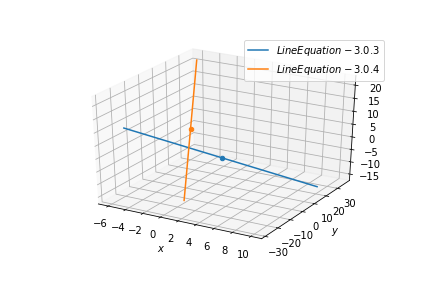
\includegraphics[width=\columnwidth]{./solutions/line_plane/74/codes/figs/Line_interest_1.png}
	\caption{Graph for equations \ref{eq:solutions/line_plane/74/codes7}}
	\label{fig:solutions/line_plane/74/codesline_equation_1}
\end{figure}


	\item 
	\begin{align}\label{eq:solutions/line_plane/74/codes12}
		\frac{x}{2} = \frac{y}{2} &= \frac{z}{1}, 
	\end{align}
	\begin{align}\label{eq:solutions/line_plane/74/codes13}
		\frac{x-5}{4} = \frac{y-2}{1} &= \frac{z-3}{8} 
	\end{align}



The above symmetric equations \ref{eq:solutions/line_plane/74/codes12}, \ref{eq:solutions/line_plane/74/codes13} can be represented in the vector form as 
\begin{align}\label{eq:solutions/line_plane/74/codes14}
	\quad \vec{r_1} &= \myvec{0\\0\\0} + \lambda_1\myvec{2\\2\\1}
	\\
	\quad \vec{r_2} &= \myvec{5\\2\\3} + \lambda_2\myvec{4\\1\\8}
\end{align}

As we have to find the angle between the vectors, we will only be taking the direction vectors into consideration. The direction vectors are $\vec{u}$ = $\myvec{2\\2\\1}$ and $\vec{v}$ = $\myvec{4\\1\\8}$. We can find the corresponding magnitude values

\begin{align}\label{eq:solutions/line_plane/74/codes16}
	\norm{\vec{u}} =\sqrt{2^{2}+2^{2}+1^{2}} =\sqrt{9}
\end{align}
\begin{align}\label{eq:solutions/line_plane/74/codes17}
	\norm{\vec{v}} =\sqrt{4^{2}+1^{2}+8^{2}} =\sqrt{81}
\end{align}

Using \ref{eq:solutions/line_plane/74/codes4}, \ref{eq:solutions/line_plane/74/codes16}, \ref{eq:solutions/line_plane/74/codes17} we get
\begin{align}
	\theta = \cos ^{-1}\frac{\myvec{2\\2\\1}^{T}\myvec{4\\1\\8}}{(\sqrt{9})(\sqrt{81})} 
	\\
	\theta = \cos ^{-1}\frac{18}{27.00}
	\\
	\theta = \cos ^{-1} (0.667)
	\\
	\theta = 48.189\degree
\end{align}

Therefore, the angle between the two lines is $48.189\degree$. See Fig. \ref{fig:solutions/line_plane/74/codesline_equation_2}


\begin{figure}
	\centering
	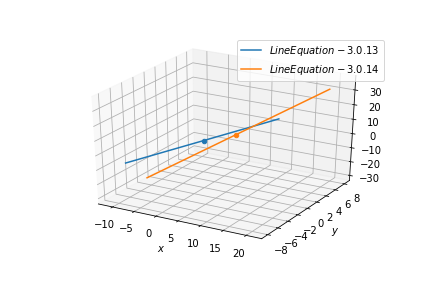
\includegraphics[width=\columnwidth]{./solutions/line_plane/74/codes/figs/Line_interest_2.png}
	\caption{Graph for equations \ref{eq:solutions/line_plane/74/codes14}}
	\label{fig:solutions/line_plane/74/codesline_equation_2}
\end{figure}
\end{enumerate}

    

\item Show that each of the given three vectors is a unit vector
\begin{align}
 \frac{1}{7}\myvec{2\\3\\6}, \frac{1}{7}\myvec{3\\-6\\2}, \frac{1}{7}\myvec{6\\2\\-3}.
\end{align}
Also,  show that they are mutually perpendicular to each other.
\\
\solution 
From theory, we understand that using dot product we can find the angle between the lines 
\begin{enumerate}
	\item 
	\begin{align}\label{eq:solutions/line_plane/74/codes:5}
		\frac{x-2}{2} = \frac{y-1}{5} &= \frac{z+3}{-3}, 
	\end{align}
	\begin{align}\label{eq:solutions/line_plane/74/codes:6}
		\frac{x+2}{-1} = \frac{y-4}{8} &= \frac{z-5}{4} 
	\end{align}


The above symmetric equations \ref{eq:solutions/line_plane/74/codes:5}, \ref{eq:solutions/line_plane/74/codes:6} can be represented in the vector form as 
\begin{align}\label{eq:solutions/line_plane/74/codes7}
	\quad \vec{r_1} &= \myvec{2\\1\\-3} + \lambda_1\myvec{2\\5\\-3}
	\\
	\quad \vec{r_2} &= \myvec{-2\\4\\5} + \lambda_2\myvec{-1\\8\\4}
\end{align}

As we have to find the angle between the vectors, we will only be taking the direction vectors into consideration. The direction vectors are $\vec{u}$ = $\myvec{2\\5\\-3}$ and $\vec{v}$ = $\myvec{-1\\8\\4}$. We can find the corresponding magnitude values

\begin{align}\label{eq:solutions/line_plane/74/codes9}
	\norm{\vec{u}} =\sqrt{2^{2}+5^{2}+(-3)^{2}} =\sqrt{38}
\end{align}
\begin{align}\label{eq:solutions/line_plane/74/codes10}
	\norm{\vec{v}} =\sqrt{(-1)^{2}+8^{2}+4^{2}} =\sqrt{81}
\end{align}

Using \ref{eq:solutions/line_plane/74/codes4}, \ref{eq:solutions/line_plane/74/codes9}, \ref{eq:solutions/line_plane/74/codes10} we get
\begin{align}
	\theta = \cos ^{-1}\frac{\myvec{2\\5\\-3}^{T}\myvec{-1\\8\\4}}{(\sqrt{38})(\sqrt{81})} 
	\\
	\theta = \cos ^{-1}\frac{26}{55.4797}
	\\
	\theta = \cos ^{-1} (0.4686)
	\\
	\theta = 62.053\degree
\end{align}

Therefore, the angle between the two lines is $62.053\degree$.See Fig. \ref{fig:solutions/line_plane/74/codesline_equation_1}

\begin{figure}
	\centering
	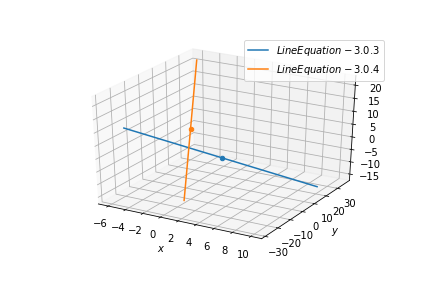
\includegraphics[width=\columnwidth]{./solutions/line_plane/74/codes/figs/Line_interest_1.png}
	\caption{Graph for equations \ref{eq:solutions/line_plane/74/codes7}}
	\label{fig:solutions/line_plane/74/codesline_equation_1}
\end{figure}


	\item 
	\begin{align}\label{eq:solutions/line_plane/74/codes12}
		\frac{x}{2} = \frac{y}{2} &= \frac{z}{1}, 
	\end{align}
	\begin{align}\label{eq:solutions/line_plane/74/codes13}
		\frac{x-5}{4} = \frac{y-2}{1} &= \frac{z-3}{8} 
	\end{align}



The above symmetric equations \ref{eq:solutions/line_plane/74/codes12}, \ref{eq:solutions/line_plane/74/codes13} can be represented in the vector form as 
\begin{align}\label{eq:solutions/line_plane/74/codes14}
	\quad \vec{r_1} &= \myvec{0\\0\\0} + \lambda_1\myvec{2\\2\\1}
	\\
	\quad \vec{r_2} &= \myvec{5\\2\\3} + \lambda_2\myvec{4\\1\\8}
\end{align}

As we have to find the angle between the vectors, we will only be taking the direction vectors into consideration. The direction vectors are $\vec{u}$ = $\myvec{2\\2\\1}$ and $\vec{v}$ = $\myvec{4\\1\\8}$. We can find the corresponding magnitude values

\begin{align}\label{eq:solutions/line_plane/74/codes16}
	\norm{\vec{u}} =\sqrt{2^{2}+2^{2}+1^{2}} =\sqrt{9}
\end{align}
\begin{align}\label{eq:solutions/line_plane/74/codes17}
	\norm{\vec{v}} =\sqrt{4^{2}+1^{2}+8^{2}} =\sqrt{81}
\end{align}

Using \ref{eq:solutions/line_plane/74/codes4}, \ref{eq:solutions/line_plane/74/codes16}, \ref{eq:solutions/line_plane/74/codes17} we get
\begin{align}
	\theta = \cos ^{-1}\frac{\myvec{2\\2\\1}^{T}\myvec{4\\1\\8}}{(\sqrt{9})(\sqrt{81})} 
	\\
	\theta = \cos ^{-1}\frac{18}{27.00}
	\\
	\theta = \cos ^{-1} (0.667)
	\\
	\theta = 48.189\degree
\end{align}

Therefore, the angle between the two lines is $48.189\degree$. See Fig. \ref{fig:solutions/line_plane/74/codesline_equation_2}


\begin{figure}
	\centering
	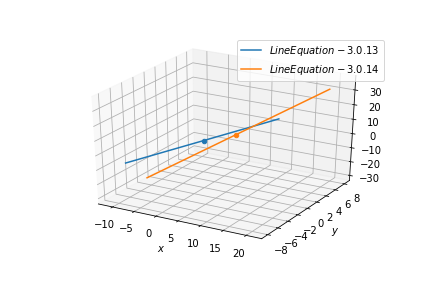
\includegraphics[width=\columnwidth]{./solutions/line_plane/74/codes/figs/Line_interest_2.png}
	\caption{Graph for equations \ref{eq:solutions/line_plane/74/codes14}}
	\label{fig:solutions/line_plane/74/codesline_equation_2}
\end{figure}
\end{enumerate}

    


\item For 
\begin{align}
\vec{a} = \myvec{2\\2\\3}, \vec{b} = \myvec{-1\\2\\1}, \vec{c} = \myvec{3\\1\\0},
\end{align}
$\brak{\vec{a}+k\vec{b}}\perp\vec{c}$.  Find $\lambda$.
\solution
From theory, we understand that using dot product we can find the angle between the lines 
\begin{enumerate}
	\item 
	\begin{align}\label{eq:solutions/line_plane/74/codes:5}
		\frac{x-2}{2} = \frac{y-1}{5} &= \frac{z+3}{-3}, 
	\end{align}
	\begin{align}\label{eq:solutions/line_plane/74/codes:6}
		\frac{x+2}{-1} = \frac{y-4}{8} &= \frac{z-5}{4} 
	\end{align}


The above symmetric equations \ref{eq:solutions/line_plane/74/codes:5}, \ref{eq:solutions/line_plane/74/codes:6} can be represented in the vector form as 
\begin{align}\label{eq:solutions/line_plane/74/codes7}
	\quad \vec{r_1} &= \myvec{2\\1\\-3} + \lambda_1\myvec{2\\5\\-3}
	\\
	\quad \vec{r_2} &= \myvec{-2\\4\\5} + \lambda_2\myvec{-1\\8\\4}
\end{align}

As we have to find the angle between the vectors, we will only be taking the direction vectors into consideration. The direction vectors are $\vec{u}$ = $\myvec{2\\5\\-3}$ and $\vec{v}$ = $\myvec{-1\\8\\4}$. We can find the corresponding magnitude values

\begin{align}\label{eq:solutions/line_plane/74/codes9}
	\norm{\vec{u}} =\sqrt{2^{2}+5^{2}+(-3)^{2}} =\sqrt{38}
\end{align}
\begin{align}\label{eq:solutions/line_plane/74/codes10}
	\norm{\vec{v}} =\sqrt{(-1)^{2}+8^{2}+4^{2}} =\sqrt{81}
\end{align}

Using \ref{eq:solutions/line_plane/74/codes4}, \ref{eq:solutions/line_plane/74/codes9}, \ref{eq:solutions/line_plane/74/codes10} we get
\begin{align}
	\theta = \cos ^{-1}\frac{\myvec{2\\5\\-3}^{T}\myvec{-1\\8\\4}}{(\sqrt{38})(\sqrt{81})} 
	\\
	\theta = \cos ^{-1}\frac{26}{55.4797}
	\\
	\theta = \cos ^{-1} (0.4686)
	\\
	\theta = 62.053\degree
\end{align}

Therefore, the angle between the two lines is $62.053\degree$.See Fig. \ref{fig:solutions/line_plane/74/codesline_equation_1}

\begin{figure}
	\centering
	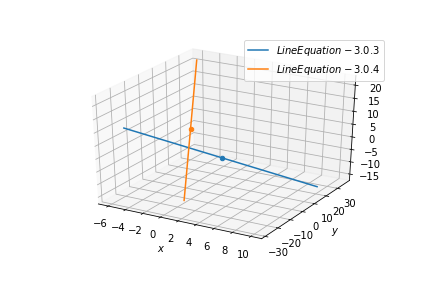
\includegraphics[width=\columnwidth]{./solutions/line_plane/74/codes/figs/Line_interest_1.png}
	\caption{Graph for equations \ref{eq:solutions/line_plane/74/codes7}}
	\label{fig:solutions/line_plane/74/codesline_equation_1}
\end{figure}


	\item 
	\begin{align}\label{eq:solutions/line_plane/74/codes12}
		\frac{x}{2} = \frac{y}{2} &= \frac{z}{1}, 
	\end{align}
	\begin{align}\label{eq:solutions/line_plane/74/codes13}
		\frac{x-5}{4} = \frac{y-2}{1} &= \frac{z-3}{8} 
	\end{align}



The above symmetric equations \ref{eq:solutions/line_plane/74/codes12}, \ref{eq:solutions/line_plane/74/codes13} can be represented in the vector form as 
\begin{align}\label{eq:solutions/line_plane/74/codes14}
	\quad \vec{r_1} &= \myvec{0\\0\\0} + \lambda_1\myvec{2\\2\\1}
	\\
	\quad \vec{r_2} &= \myvec{5\\2\\3} + \lambda_2\myvec{4\\1\\8}
\end{align}

As we have to find the angle between the vectors, we will only be taking the direction vectors into consideration. The direction vectors are $\vec{u}$ = $\myvec{2\\2\\1}$ and $\vec{v}$ = $\myvec{4\\1\\8}$. We can find the corresponding magnitude values

\begin{align}\label{eq:solutions/line_plane/74/codes16}
	\norm{\vec{u}} =\sqrt{2^{2}+2^{2}+1^{2}} =\sqrt{9}
\end{align}
\begin{align}\label{eq:solutions/line_plane/74/codes17}
	\norm{\vec{v}} =\sqrt{4^{2}+1^{2}+8^{2}} =\sqrt{81}
\end{align}

Using \ref{eq:solutions/line_plane/74/codes4}, \ref{eq:solutions/line_plane/74/codes16}, \ref{eq:solutions/line_plane/74/codes17} we get
\begin{align}
	\theta = \cos ^{-1}\frac{\myvec{2\\2\\1}^{T}\myvec{4\\1\\8}}{(\sqrt{9})(\sqrt{81})} 
	\\
	\theta = \cos ^{-1}\frac{18}{27.00}
	\\
	\theta = \cos ^{-1} (0.667)
	\\
	\theta = 48.189\degree
\end{align}

Therefore, the angle between the two lines is $48.189\degree$. See Fig. \ref{fig:solutions/line_plane/74/codesline_equation_2}


\begin{figure}
	\centering
	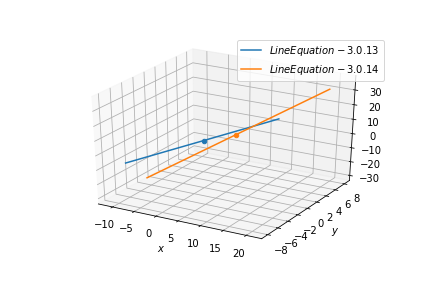
\includegraphics[width=\columnwidth]{./solutions/line_plane/74/codes/figs/Line_interest_2.png}
	\caption{Graph for equations \ref{eq:solutions/line_plane/74/codes14}}
	\label{fig:solutions/line_plane/74/codesline_equation_2}
\end{figure}
\end{enumerate}

    


\item Find ${\vec{a} \times \vec{b}}$ if 
\begin{align}
\vec{a}=\myvec{1\\-7\\7},
\vec{b}=\myvec{3\\-2\\2}.
\end{align}
\\
\solution 
From theory, we understand that using dot product we can find the angle between the lines 
\begin{enumerate}
	\item 
	\begin{align}\label{eq:solutions/line_plane/74/codes:5}
		\frac{x-2}{2} = \frac{y-1}{5} &= \frac{z+3}{-3}, 
	\end{align}
	\begin{align}\label{eq:solutions/line_plane/74/codes:6}
		\frac{x+2}{-1} = \frac{y-4}{8} &= \frac{z-5}{4} 
	\end{align}


The above symmetric equations \ref{eq:solutions/line_plane/74/codes:5}, \ref{eq:solutions/line_plane/74/codes:6} can be represented in the vector form as 
\begin{align}\label{eq:solutions/line_plane/74/codes7}
	\quad \vec{r_1} &= \myvec{2\\1\\-3} + \lambda_1\myvec{2\\5\\-3}
	\\
	\quad \vec{r_2} &= \myvec{-2\\4\\5} + \lambda_2\myvec{-1\\8\\4}
\end{align}

As we have to find the angle between the vectors, we will only be taking the direction vectors into consideration. The direction vectors are $\vec{u}$ = $\myvec{2\\5\\-3}$ and $\vec{v}$ = $\myvec{-1\\8\\4}$. We can find the corresponding magnitude values

\begin{align}\label{eq:solutions/line_plane/74/codes9}
	\norm{\vec{u}} =\sqrt{2^{2}+5^{2}+(-3)^{2}} =\sqrt{38}
\end{align}
\begin{align}\label{eq:solutions/line_plane/74/codes10}
	\norm{\vec{v}} =\sqrt{(-1)^{2}+8^{2}+4^{2}} =\sqrt{81}
\end{align}

Using \ref{eq:solutions/line_plane/74/codes4}, \ref{eq:solutions/line_plane/74/codes9}, \ref{eq:solutions/line_plane/74/codes10} we get
\begin{align}
	\theta = \cos ^{-1}\frac{\myvec{2\\5\\-3}^{T}\myvec{-1\\8\\4}}{(\sqrt{38})(\sqrt{81})} 
	\\
	\theta = \cos ^{-1}\frac{26}{55.4797}
	\\
	\theta = \cos ^{-1} (0.4686)
	\\
	\theta = 62.053\degree
\end{align}

Therefore, the angle between the two lines is $62.053\degree$.See Fig. \ref{fig:solutions/line_plane/74/codesline_equation_1}

\begin{figure}
	\centering
	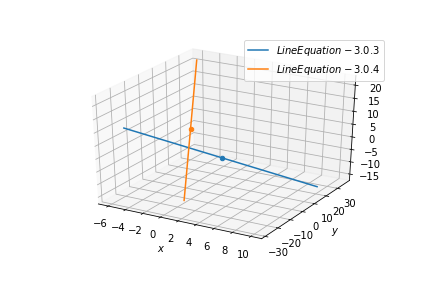
\includegraphics[width=\columnwidth]{./solutions/line_plane/74/codes/figs/Line_interest_1.png}
	\caption{Graph for equations \ref{eq:solutions/line_plane/74/codes7}}
	\label{fig:solutions/line_plane/74/codesline_equation_1}
\end{figure}


	\item 
	\begin{align}\label{eq:solutions/line_plane/74/codes12}
		\frac{x}{2} = \frac{y}{2} &= \frac{z}{1}, 
	\end{align}
	\begin{align}\label{eq:solutions/line_plane/74/codes13}
		\frac{x-5}{4} = \frac{y-2}{1} &= \frac{z-3}{8} 
	\end{align}



The above symmetric equations \ref{eq:solutions/line_plane/74/codes12}, \ref{eq:solutions/line_plane/74/codes13} can be represented in the vector form as 
\begin{align}\label{eq:solutions/line_plane/74/codes14}
	\quad \vec{r_1} &= \myvec{0\\0\\0} + \lambda_1\myvec{2\\2\\1}
	\\
	\quad \vec{r_2} &= \myvec{5\\2\\3} + \lambda_2\myvec{4\\1\\8}
\end{align}

As we have to find the angle between the vectors, we will only be taking the direction vectors into consideration. The direction vectors are $\vec{u}$ = $\myvec{2\\2\\1}$ and $\vec{v}$ = $\myvec{4\\1\\8}$. We can find the corresponding magnitude values

\begin{align}\label{eq:solutions/line_plane/74/codes16}
	\norm{\vec{u}} =\sqrt{2^{2}+2^{2}+1^{2}} =\sqrt{9}
\end{align}
\begin{align}\label{eq:solutions/line_plane/74/codes17}
	\norm{\vec{v}} =\sqrt{4^{2}+1^{2}+8^{2}} =\sqrt{81}
\end{align}

Using \ref{eq:solutions/line_plane/74/codes4}, \ref{eq:solutions/line_plane/74/codes16}, \ref{eq:solutions/line_plane/74/codes17} we get
\begin{align}
	\theta = \cos ^{-1}\frac{\myvec{2\\2\\1}^{T}\myvec{4\\1\\8}}{(\sqrt{9})(\sqrt{81})} 
	\\
	\theta = \cos ^{-1}\frac{18}{27.00}
	\\
	\theta = \cos ^{-1} (0.667)
	\\
	\theta = 48.189\degree
\end{align}

Therefore, the angle between the two lines is $48.189\degree$. See Fig. \ref{fig:solutions/line_plane/74/codesline_equation_2}


\begin{figure}
	\centering
	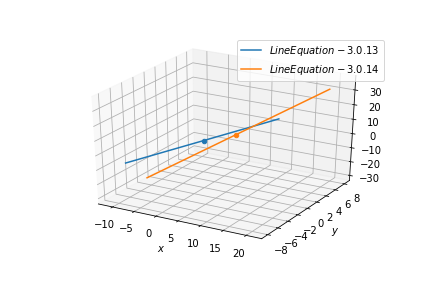
\includegraphics[width=\columnwidth]{./solutions/line_plane/74/codes/figs/Line_interest_2.png}
	\caption{Graph for equations \ref{eq:solutions/line_plane/74/codes14}}
	\label{fig:solutions/line_plane/74/codesline_equation_2}
\end{figure}
\end{enumerate}

    

\item Find a unit vector perpendicular to each of the vectors 
$\vec{a}+\vec{b}$ and $\vec{a}-\vec{b}$, where 
\begin{align}
\vec{a}=\myvec{3\\2\\2},
\vec{b}=\myvec{1\\2\\-2}.
\end{align}
\\
\solution 
From theory, we understand that using dot product we can find the angle between the lines 
\begin{enumerate}
	\item 
	\begin{align}\label{eq:solutions/line_plane/74/codes:5}
		\frac{x-2}{2} = \frac{y-1}{5} &= \frac{z+3}{-3}, 
	\end{align}
	\begin{align}\label{eq:solutions/line_plane/74/codes:6}
		\frac{x+2}{-1} = \frac{y-4}{8} &= \frac{z-5}{4} 
	\end{align}


The above symmetric equations \ref{eq:solutions/line_plane/74/codes:5}, \ref{eq:solutions/line_plane/74/codes:6} can be represented in the vector form as 
\begin{align}\label{eq:solutions/line_plane/74/codes7}
	\quad \vec{r_1} &= \myvec{2\\1\\-3} + \lambda_1\myvec{2\\5\\-3}
	\\
	\quad \vec{r_2} &= \myvec{-2\\4\\5} + \lambda_2\myvec{-1\\8\\4}
\end{align}

As we have to find the angle between the vectors, we will only be taking the direction vectors into consideration. The direction vectors are $\vec{u}$ = $\myvec{2\\5\\-3}$ and $\vec{v}$ = $\myvec{-1\\8\\4}$. We can find the corresponding magnitude values

\begin{align}\label{eq:solutions/line_plane/74/codes9}
	\norm{\vec{u}} =\sqrt{2^{2}+5^{2}+(-3)^{2}} =\sqrt{38}
\end{align}
\begin{align}\label{eq:solutions/line_plane/74/codes10}
	\norm{\vec{v}} =\sqrt{(-1)^{2}+8^{2}+4^{2}} =\sqrt{81}
\end{align}

Using \ref{eq:solutions/line_plane/74/codes4}, \ref{eq:solutions/line_plane/74/codes9}, \ref{eq:solutions/line_plane/74/codes10} we get
\begin{align}
	\theta = \cos ^{-1}\frac{\myvec{2\\5\\-3}^{T}\myvec{-1\\8\\4}}{(\sqrt{38})(\sqrt{81})} 
	\\
	\theta = \cos ^{-1}\frac{26}{55.4797}
	\\
	\theta = \cos ^{-1} (0.4686)
	\\
	\theta = 62.053\degree
\end{align}

Therefore, the angle between the two lines is $62.053\degree$.See Fig. \ref{fig:solutions/line_plane/74/codesline_equation_1}

\begin{figure}
	\centering
	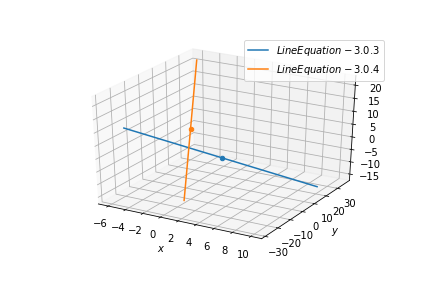
\includegraphics[width=\columnwidth]{./solutions/line_plane/74/codes/figs/Line_interest_1.png}
	\caption{Graph for equations \ref{eq:solutions/line_plane/74/codes7}}
	\label{fig:solutions/line_plane/74/codesline_equation_1}
\end{figure}


	\item 
	\begin{align}\label{eq:solutions/line_plane/74/codes12}
		\frac{x}{2} = \frac{y}{2} &= \frac{z}{1}, 
	\end{align}
	\begin{align}\label{eq:solutions/line_plane/74/codes13}
		\frac{x-5}{4} = \frac{y-2}{1} &= \frac{z-3}{8} 
	\end{align}



The above symmetric equations \ref{eq:solutions/line_plane/74/codes12}, \ref{eq:solutions/line_plane/74/codes13} can be represented in the vector form as 
\begin{align}\label{eq:solutions/line_plane/74/codes14}
	\quad \vec{r_1} &= \myvec{0\\0\\0} + \lambda_1\myvec{2\\2\\1}
	\\
	\quad \vec{r_2} &= \myvec{5\\2\\3} + \lambda_2\myvec{4\\1\\8}
\end{align}

As we have to find the angle between the vectors, we will only be taking the direction vectors into consideration. The direction vectors are $\vec{u}$ = $\myvec{2\\2\\1}$ and $\vec{v}$ = $\myvec{4\\1\\8}$. We can find the corresponding magnitude values

\begin{align}\label{eq:solutions/line_plane/74/codes16}
	\norm{\vec{u}} =\sqrt{2^{2}+2^{2}+1^{2}} =\sqrt{9}
\end{align}
\begin{align}\label{eq:solutions/line_plane/74/codes17}
	\norm{\vec{v}} =\sqrt{4^{2}+1^{2}+8^{2}} =\sqrt{81}
\end{align}

Using \ref{eq:solutions/line_plane/74/codes4}, \ref{eq:solutions/line_plane/74/codes16}, \ref{eq:solutions/line_plane/74/codes17} we get
\begin{align}
	\theta = \cos ^{-1}\frac{\myvec{2\\2\\1}^{T}\myvec{4\\1\\8}}{(\sqrt{9})(\sqrt{81})} 
	\\
	\theta = \cos ^{-1}\frac{18}{27.00}
	\\
	\theta = \cos ^{-1} (0.667)
	\\
	\theta = 48.189\degree
\end{align}

Therefore, the angle between the two lines is $48.189\degree$. See Fig. \ref{fig:solutions/line_plane/74/codesline_equation_2}


\begin{figure}
	\centering
	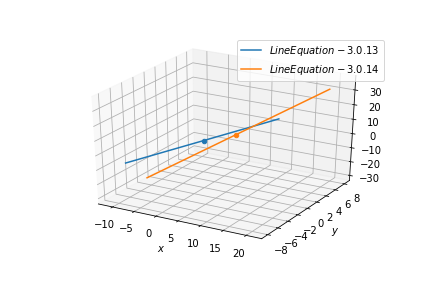
\includegraphics[width=\columnwidth]{./solutions/line_plane/74/codes/figs/Line_interest_2.png}
	\caption{Graph for equations \ref{eq:solutions/line_plane/74/codes14}}
	\label{fig:solutions/line_plane/74/codesline_equation_2}
\end{figure}
\end{enumerate}

    

\item  If 
$
\vec{a}=\myvec{1\\1\\1},
\vec{b}=\myvec{2\\-1\\3},
\vec{c}=\myvec{1\\-2\\1},
$
find a unit vector parallel to the vector $2\vec{a}-\vec{b}+3\vec{c}$.
\\
\solution 
From theory, we understand that using dot product we can find the angle between the lines 
\begin{enumerate}
	\item 
	\begin{align}\label{eq:solutions/line_plane/74/codes:5}
		\frac{x-2}{2} = \frac{y-1}{5} &= \frac{z+3}{-3}, 
	\end{align}
	\begin{align}\label{eq:solutions/line_plane/74/codes:6}
		\frac{x+2}{-1} = \frac{y-4}{8} &= \frac{z-5}{4} 
	\end{align}


The above symmetric equations \ref{eq:solutions/line_plane/74/codes:5}, \ref{eq:solutions/line_plane/74/codes:6} can be represented in the vector form as 
\begin{align}\label{eq:solutions/line_plane/74/codes7}
	\quad \vec{r_1} &= \myvec{2\\1\\-3} + \lambda_1\myvec{2\\5\\-3}
	\\
	\quad \vec{r_2} &= \myvec{-2\\4\\5} + \lambda_2\myvec{-1\\8\\4}
\end{align}

As we have to find the angle between the vectors, we will only be taking the direction vectors into consideration. The direction vectors are $\vec{u}$ = $\myvec{2\\5\\-3}$ and $\vec{v}$ = $\myvec{-1\\8\\4}$. We can find the corresponding magnitude values

\begin{align}\label{eq:solutions/line_plane/74/codes9}
	\norm{\vec{u}} =\sqrt{2^{2}+5^{2}+(-3)^{2}} =\sqrt{38}
\end{align}
\begin{align}\label{eq:solutions/line_plane/74/codes10}
	\norm{\vec{v}} =\sqrt{(-1)^{2}+8^{2}+4^{2}} =\sqrt{81}
\end{align}

Using \ref{eq:solutions/line_plane/74/codes4}, \ref{eq:solutions/line_plane/74/codes9}, \ref{eq:solutions/line_plane/74/codes10} we get
\begin{align}
	\theta = \cos ^{-1}\frac{\myvec{2\\5\\-3}^{T}\myvec{-1\\8\\4}}{(\sqrt{38})(\sqrt{81})} 
	\\
	\theta = \cos ^{-1}\frac{26}{55.4797}
	\\
	\theta = \cos ^{-1} (0.4686)
	\\
	\theta = 62.053\degree
\end{align}

Therefore, the angle between the two lines is $62.053\degree$.See Fig. \ref{fig:solutions/line_plane/74/codesline_equation_1}

\begin{figure}
	\centering
	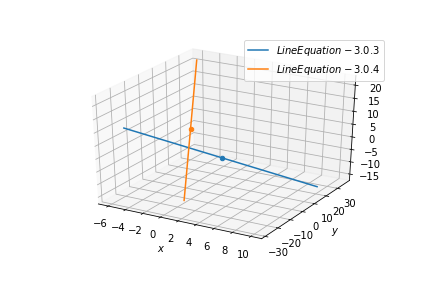
\includegraphics[width=\columnwidth]{./solutions/line_plane/74/codes/figs/Line_interest_1.png}
	\caption{Graph for equations \ref{eq:solutions/line_plane/74/codes7}}
	\label{fig:solutions/line_plane/74/codesline_equation_1}
\end{figure}


	\item 
	\begin{align}\label{eq:solutions/line_plane/74/codes12}
		\frac{x}{2} = \frac{y}{2} &= \frac{z}{1}, 
	\end{align}
	\begin{align}\label{eq:solutions/line_plane/74/codes13}
		\frac{x-5}{4} = \frac{y-2}{1} &= \frac{z-3}{8} 
	\end{align}



The above symmetric equations \ref{eq:solutions/line_plane/74/codes12}, \ref{eq:solutions/line_plane/74/codes13} can be represented in the vector form as 
\begin{align}\label{eq:solutions/line_plane/74/codes14}
	\quad \vec{r_1} &= \myvec{0\\0\\0} + \lambda_1\myvec{2\\2\\1}
	\\
	\quad \vec{r_2} &= \myvec{5\\2\\3} + \lambda_2\myvec{4\\1\\8}
\end{align}

As we have to find the angle between the vectors, we will only be taking the direction vectors into consideration. The direction vectors are $\vec{u}$ = $\myvec{2\\2\\1}$ and $\vec{v}$ = $\myvec{4\\1\\8}$. We can find the corresponding magnitude values

\begin{align}\label{eq:solutions/line_plane/74/codes16}
	\norm{\vec{u}} =\sqrt{2^{2}+2^{2}+1^{2}} =\sqrt{9}
\end{align}
\begin{align}\label{eq:solutions/line_plane/74/codes17}
	\norm{\vec{v}} =\sqrt{4^{2}+1^{2}+8^{2}} =\sqrt{81}
\end{align}

Using \ref{eq:solutions/line_plane/74/codes4}, \ref{eq:solutions/line_plane/74/codes16}, \ref{eq:solutions/line_plane/74/codes17} we get
\begin{align}
	\theta = \cos ^{-1}\frac{\myvec{2\\2\\1}^{T}\myvec{4\\1\\8}}{(\sqrt{9})(\sqrt{81})} 
	\\
	\theta = \cos ^{-1}\frac{18}{27.00}
	\\
	\theta = \cos ^{-1} (0.667)
	\\
	\theta = 48.189\degree
\end{align}

Therefore, the angle between the two lines is $48.189\degree$. See Fig. \ref{fig:solutions/line_plane/74/codesline_equation_2}


\begin{figure}
	\centering
	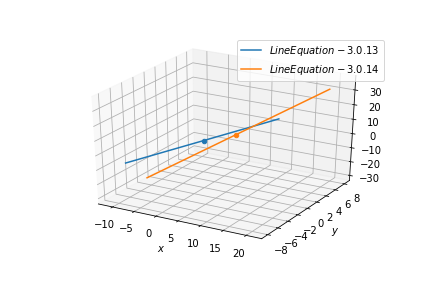
\includegraphics[width=\columnwidth]{./solutions/line_plane/74/codes/figs/Line_interest_2.png}
	\caption{Graph for equations \ref{eq:solutions/line_plane/74/codes14}}
	\label{fig:solutions/line_plane/74/codesline_equation_2}
\end{figure}
\end{enumerate}

    


\item Find a vector of magnitude 5 units, and parallel to the resultant of the vectors 
$
\vec{a}=\myvec{2\\3\\-1},
\vec{b}=\myvec{1\\-2\\1},
$
\\
\solution 
From theory, we understand that using dot product we can find the angle between the lines 
\begin{enumerate}
	\item 
	\begin{align}\label{eq:solutions/line_plane/74/codes:5}
		\frac{x-2}{2} = \frac{y-1}{5} &= \frac{z+3}{-3}, 
	\end{align}
	\begin{align}\label{eq:solutions/line_plane/74/codes:6}
		\frac{x+2}{-1} = \frac{y-4}{8} &= \frac{z-5}{4} 
	\end{align}


The above symmetric equations \ref{eq:solutions/line_plane/74/codes:5}, \ref{eq:solutions/line_plane/74/codes:6} can be represented in the vector form as 
\begin{align}\label{eq:solutions/line_plane/74/codes7}
	\quad \vec{r_1} &= \myvec{2\\1\\-3} + \lambda_1\myvec{2\\5\\-3}
	\\
	\quad \vec{r_2} &= \myvec{-2\\4\\5} + \lambda_2\myvec{-1\\8\\4}
\end{align}

As we have to find the angle between the vectors, we will only be taking the direction vectors into consideration. The direction vectors are $\vec{u}$ = $\myvec{2\\5\\-3}$ and $\vec{v}$ = $\myvec{-1\\8\\4}$. We can find the corresponding magnitude values

\begin{align}\label{eq:solutions/line_plane/74/codes9}
	\norm{\vec{u}} =\sqrt{2^{2}+5^{2}+(-3)^{2}} =\sqrt{38}
\end{align}
\begin{align}\label{eq:solutions/line_plane/74/codes10}
	\norm{\vec{v}} =\sqrt{(-1)^{2}+8^{2}+4^{2}} =\sqrt{81}
\end{align}

Using \ref{eq:solutions/line_plane/74/codes4}, \ref{eq:solutions/line_plane/74/codes9}, \ref{eq:solutions/line_plane/74/codes10} we get
\begin{align}
	\theta = \cos ^{-1}\frac{\myvec{2\\5\\-3}^{T}\myvec{-1\\8\\4}}{(\sqrt{38})(\sqrt{81})} 
	\\
	\theta = \cos ^{-1}\frac{26}{55.4797}
	\\
	\theta = \cos ^{-1} (0.4686)
	\\
	\theta = 62.053\degree
\end{align}

Therefore, the angle between the two lines is $62.053\degree$.See Fig. \ref{fig:solutions/line_plane/74/codesline_equation_1}

\begin{figure}
	\centering
	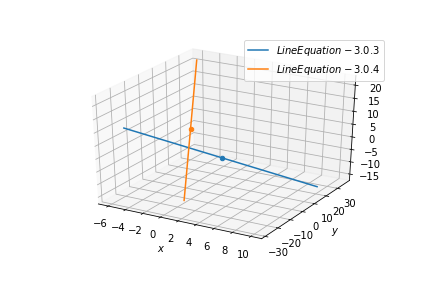
\includegraphics[width=\columnwidth]{./solutions/line_plane/74/codes/figs/Line_interest_1.png}
	\caption{Graph for equations \ref{eq:solutions/line_plane/74/codes7}}
	\label{fig:solutions/line_plane/74/codesline_equation_1}
\end{figure}


	\item 
	\begin{align}\label{eq:solutions/line_plane/74/codes12}
		\frac{x}{2} = \frac{y}{2} &= \frac{z}{1}, 
	\end{align}
	\begin{align}\label{eq:solutions/line_plane/74/codes13}
		\frac{x-5}{4} = \frac{y-2}{1} &= \frac{z-3}{8} 
	\end{align}



The above symmetric equations \ref{eq:solutions/line_plane/74/codes12}, \ref{eq:solutions/line_plane/74/codes13} can be represented in the vector form as 
\begin{align}\label{eq:solutions/line_plane/74/codes14}
	\quad \vec{r_1} &= \myvec{0\\0\\0} + \lambda_1\myvec{2\\2\\1}
	\\
	\quad \vec{r_2} &= \myvec{5\\2\\3} + \lambda_2\myvec{4\\1\\8}
\end{align}

As we have to find the angle between the vectors, we will only be taking the direction vectors into consideration. The direction vectors are $\vec{u}$ = $\myvec{2\\2\\1}$ and $\vec{v}$ = $\myvec{4\\1\\8}$. We can find the corresponding magnitude values

\begin{align}\label{eq:solutions/line_plane/74/codes16}
	\norm{\vec{u}} =\sqrt{2^{2}+2^{2}+1^{2}} =\sqrt{9}
\end{align}
\begin{align}\label{eq:solutions/line_plane/74/codes17}
	\norm{\vec{v}} =\sqrt{4^{2}+1^{2}+8^{2}} =\sqrt{81}
\end{align}

Using \ref{eq:solutions/line_plane/74/codes4}, \ref{eq:solutions/line_plane/74/codes16}, \ref{eq:solutions/line_plane/74/codes17} we get
\begin{align}
	\theta = \cos ^{-1}\frac{\myvec{2\\2\\1}^{T}\myvec{4\\1\\8}}{(\sqrt{9})(\sqrt{81})} 
	\\
	\theta = \cos ^{-1}\frac{18}{27.00}
	\\
	\theta = \cos ^{-1} (0.667)
	\\
	\theta = 48.189\degree
\end{align}

Therefore, the angle between the two lines is $48.189\degree$. See Fig. \ref{fig:solutions/line_plane/74/codesline_equation_2}


\begin{figure}
	\centering
	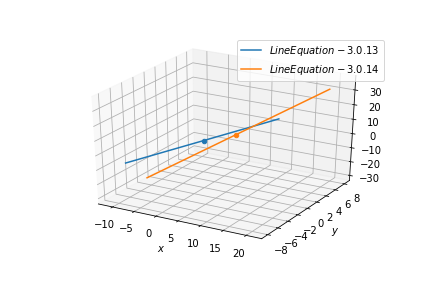
\includegraphics[width=\columnwidth]{./solutions/line_plane/74/codes/figs/Line_interest_2.png}
	\caption{Graph for equations \ref{eq:solutions/line_plane/74/codes14}}
	\label{fig:solutions/line_plane/74/codesline_equation_2}
\end{figure}
\end{enumerate}

    

\item Show that the unit direction vector inclined equally to the coordinate axes is $\myvec{\frac{1}{\sqrt{3}}\\\frac{1}{\sqrt{3}}\\ \frac{1}{\sqrt{3}}}$.
\\
\solution 
From theory, we understand that using dot product we can find the angle between the lines 
\begin{enumerate}
	\item 
	\begin{align}\label{eq:solutions/line_plane/74/codes:5}
		\frac{x-2}{2} = \frac{y-1}{5} &= \frac{z+3}{-3}, 
	\end{align}
	\begin{align}\label{eq:solutions/line_plane/74/codes:6}
		\frac{x+2}{-1} = \frac{y-4}{8} &= \frac{z-5}{4} 
	\end{align}


The above symmetric equations \ref{eq:solutions/line_plane/74/codes:5}, \ref{eq:solutions/line_plane/74/codes:6} can be represented in the vector form as 
\begin{align}\label{eq:solutions/line_plane/74/codes7}
	\quad \vec{r_1} &= \myvec{2\\1\\-3} + \lambda_1\myvec{2\\5\\-3}
	\\
	\quad \vec{r_2} &= \myvec{-2\\4\\5} + \lambda_2\myvec{-1\\8\\4}
\end{align}

As we have to find the angle between the vectors, we will only be taking the direction vectors into consideration. The direction vectors are $\vec{u}$ = $\myvec{2\\5\\-3}$ and $\vec{v}$ = $\myvec{-1\\8\\4}$. We can find the corresponding magnitude values

\begin{align}\label{eq:solutions/line_plane/74/codes9}
	\norm{\vec{u}} =\sqrt{2^{2}+5^{2}+(-3)^{2}} =\sqrt{38}
\end{align}
\begin{align}\label{eq:solutions/line_plane/74/codes10}
	\norm{\vec{v}} =\sqrt{(-1)^{2}+8^{2}+4^{2}} =\sqrt{81}
\end{align}

Using \ref{eq:solutions/line_plane/74/codes4}, \ref{eq:solutions/line_plane/74/codes9}, \ref{eq:solutions/line_plane/74/codes10} we get
\begin{align}
	\theta = \cos ^{-1}\frac{\myvec{2\\5\\-3}^{T}\myvec{-1\\8\\4}}{(\sqrt{38})(\sqrt{81})} 
	\\
	\theta = \cos ^{-1}\frac{26}{55.4797}
	\\
	\theta = \cos ^{-1} (0.4686)
	\\
	\theta = 62.053\degree
\end{align}

Therefore, the angle between the two lines is $62.053\degree$.See Fig. \ref{fig:solutions/line_plane/74/codesline_equation_1}

\begin{figure}
	\centering
	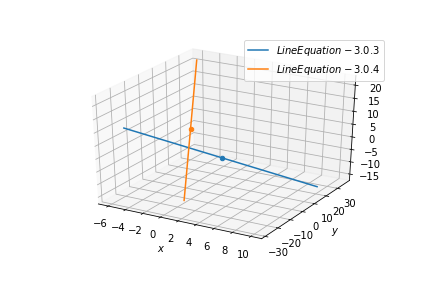
\includegraphics[width=\columnwidth]{./solutions/line_plane/74/codes/figs/Line_interest_1.png}
	\caption{Graph for equations \ref{eq:solutions/line_plane/74/codes7}}
	\label{fig:solutions/line_plane/74/codesline_equation_1}
\end{figure}


	\item 
	\begin{align}\label{eq:solutions/line_plane/74/codes12}
		\frac{x}{2} = \frac{y}{2} &= \frac{z}{1}, 
	\end{align}
	\begin{align}\label{eq:solutions/line_plane/74/codes13}
		\frac{x-5}{4} = \frac{y-2}{1} &= \frac{z-3}{8} 
	\end{align}



The above symmetric equations \ref{eq:solutions/line_plane/74/codes12}, \ref{eq:solutions/line_plane/74/codes13} can be represented in the vector form as 
\begin{align}\label{eq:solutions/line_plane/74/codes14}
	\quad \vec{r_1} &= \myvec{0\\0\\0} + \lambda_1\myvec{2\\2\\1}
	\\
	\quad \vec{r_2} &= \myvec{5\\2\\3} + \lambda_2\myvec{4\\1\\8}
\end{align}

As we have to find the angle between the vectors, we will only be taking the direction vectors into consideration. The direction vectors are $\vec{u}$ = $\myvec{2\\2\\1}$ and $\vec{v}$ = $\myvec{4\\1\\8}$. We can find the corresponding magnitude values

\begin{align}\label{eq:solutions/line_plane/74/codes16}
	\norm{\vec{u}} =\sqrt{2^{2}+2^{2}+1^{2}} =\sqrt{9}
\end{align}
\begin{align}\label{eq:solutions/line_plane/74/codes17}
	\norm{\vec{v}} =\sqrt{4^{2}+1^{2}+8^{2}} =\sqrt{81}
\end{align}

Using \ref{eq:solutions/line_plane/74/codes4}, \ref{eq:solutions/line_plane/74/codes16}, \ref{eq:solutions/line_plane/74/codes17} we get
\begin{align}
	\theta = \cos ^{-1}\frac{\myvec{2\\2\\1}^{T}\myvec{4\\1\\8}}{(\sqrt{9})(\sqrt{81})} 
	\\
	\theta = \cos ^{-1}\frac{18}{27.00}
	\\
	\theta = \cos ^{-1} (0.667)
	\\
	\theta = 48.189\degree
\end{align}

Therefore, the angle between the two lines is $48.189\degree$. See Fig. \ref{fig:solutions/line_plane/74/codesline_equation_2}


\begin{figure}
	\centering
	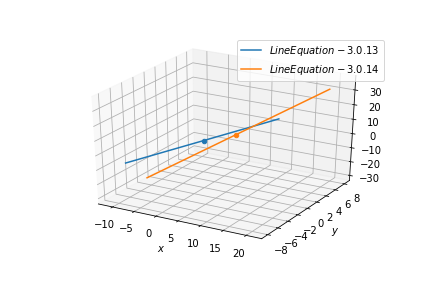
\includegraphics[width=\columnwidth]{./solutions/line_plane/74/codes/figs/Line_interest_2.png}
	\caption{Graph for equations \ref{eq:solutions/line_plane/74/codes14}}
	\label{fig:solutions/line_plane/74/codesline_equation_2}
\end{figure}
\end{enumerate}

    

\item Let 
$
\vec{a}=\myvec{1\\4\\2},
\vec{b}=\myvec{3\\-2\\7} \text{ and }
\vec{c}=\myvec{2\\-1\\4}.
$
Find a vector $\vec{d}$ such that $\vec{d}\perp\vec{a},\vec{d}\perp\vec{b}$ and $\vec{d}^T\vec{c} = 15$.
\\
\solution 
From theory, we understand that using dot product we can find the angle between the lines 
\begin{enumerate}
	\item 
	\begin{align}\label{eq:solutions/line_plane/74/codes:5}
		\frac{x-2}{2} = \frac{y-1}{5} &= \frac{z+3}{-3}, 
	\end{align}
	\begin{align}\label{eq:solutions/line_plane/74/codes:6}
		\frac{x+2}{-1} = \frac{y-4}{8} &= \frac{z-5}{4} 
	\end{align}


The above symmetric equations \ref{eq:solutions/line_plane/74/codes:5}, \ref{eq:solutions/line_plane/74/codes:6} can be represented in the vector form as 
\begin{align}\label{eq:solutions/line_plane/74/codes7}
	\quad \vec{r_1} &= \myvec{2\\1\\-3} + \lambda_1\myvec{2\\5\\-3}
	\\
	\quad \vec{r_2} &= \myvec{-2\\4\\5} + \lambda_2\myvec{-1\\8\\4}
\end{align}

As we have to find the angle between the vectors, we will only be taking the direction vectors into consideration. The direction vectors are $\vec{u}$ = $\myvec{2\\5\\-3}$ and $\vec{v}$ = $\myvec{-1\\8\\4}$. We can find the corresponding magnitude values

\begin{align}\label{eq:solutions/line_plane/74/codes9}
	\norm{\vec{u}} =\sqrt{2^{2}+5^{2}+(-3)^{2}} =\sqrt{38}
\end{align}
\begin{align}\label{eq:solutions/line_plane/74/codes10}
	\norm{\vec{v}} =\sqrt{(-1)^{2}+8^{2}+4^{2}} =\sqrt{81}
\end{align}

Using \ref{eq:solutions/line_plane/74/codes4}, \ref{eq:solutions/line_plane/74/codes9}, \ref{eq:solutions/line_plane/74/codes10} we get
\begin{align}
	\theta = \cos ^{-1}\frac{\myvec{2\\5\\-3}^{T}\myvec{-1\\8\\4}}{(\sqrt{38})(\sqrt{81})} 
	\\
	\theta = \cos ^{-1}\frac{26}{55.4797}
	\\
	\theta = \cos ^{-1} (0.4686)
	\\
	\theta = 62.053\degree
\end{align}

Therefore, the angle between the two lines is $62.053\degree$.See Fig. \ref{fig:solutions/line_plane/74/codesline_equation_1}

\begin{figure}
	\centering
	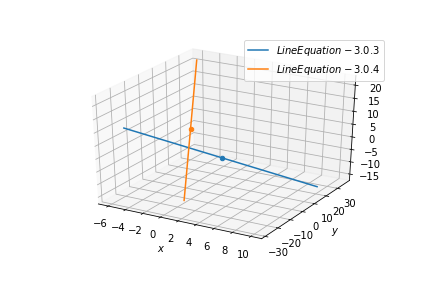
\includegraphics[width=\columnwidth]{./solutions/line_plane/74/codes/figs/Line_interest_1.png}
	\caption{Graph for equations \ref{eq:solutions/line_plane/74/codes7}}
	\label{fig:solutions/line_plane/74/codesline_equation_1}
\end{figure}


	\item 
	\begin{align}\label{eq:solutions/line_plane/74/codes12}
		\frac{x}{2} = \frac{y}{2} &= \frac{z}{1}, 
	\end{align}
	\begin{align}\label{eq:solutions/line_plane/74/codes13}
		\frac{x-5}{4} = \frac{y-2}{1} &= \frac{z-3}{8} 
	\end{align}



The above symmetric equations \ref{eq:solutions/line_plane/74/codes12}, \ref{eq:solutions/line_plane/74/codes13} can be represented in the vector form as 
\begin{align}\label{eq:solutions/line_plane/74/codes14}
	\quad \vec{r_1} &= \myvec{0\\0\\0} + \lambda_1\myvec{2\\2\\1}
	\\
	\quad \vec{r_2} &= \myvec{5\\2\\3} + \lambda_2\myvec{4\\1\\8}
\end{align}

As we have to find the angle between the vectors, we will only be taking the direction vectors into consideration. The direction vectors are $\vec{u}$ = $\myvec{2\\2\\1}$ and $\vec{v}$ = $\myvec{4\\1\\8}$. We can find the corresponding magnitude values

\begin{align}\label{eq:solutions/line_plane/74/codes16}
	\norm{\vec{u}} =\sqrt{2^{2}+2^{2}+1^{2}} =\sqrt{9}
\end{align}
\begin{align}\label{eq:solutions/line_plane/74/codes17}
	\norm{\vec{v}} =\sqrt{4^{2}+1^{2}+8^{2}} =\sqrt{81}
\end{align}

Using \ref{eq:solutions/line_plane/74/codes4}, \ref{eq:solutions/line_plane/74/codes16}, \ref{eq:solutions/line_plane/74/codes17} we get
\begin{align}
	\theta = \cos ^{-1}\frac{\myvec{2\\2\\1}^{T}\myvec{4\\1\\8}}{(\sqrt{9})(\sqrt{81})} 
	\\
	\theta = \cos ^{-1}\frac{18}{27.00}
	\\
	\theta = \cos ^{-1} (0.667)
	\\
	\theta = 48.189\degree
\end{align}

Therefore, the angle between the two lines is $48.189\degree$. See Fig. \ref{fig:solutions/line_plane/74/codesline_equation_2}


\begin{figure}
	\centering
	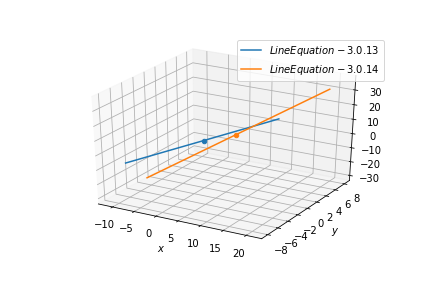
\includegraphics[width=\columnwidth]{./solutions/line_plane/74/codes/figs/Line_interest_2.png}
	\caption{Graph for equations \ref{eq:solutions/line_plane/74/codes14}}
	\label{fig:solutions/line_plane/74/codesline_equation_2}
\end{figure}
\end{enumerate}

    

\item The scalar product of \myvec{1\\1\\1} with a unit vector along the sum  of the vectors \myvec{2\\4\\-5} and \myvec{\lambda\\2\\3} is unity.  Find the value of $\lambda$.
\item The value of 
\begin{multline}
\myvec{1\\0\\0}^T\brak{\myvec{0\\1\\0}\times \myvec{0\\0\\1}}
+\myvec{0\\1\\0}^T\brak{\myvec{1\\0\\0}\times \myvec{0\\0\\1}}
\\
+\myvec{0\\0\\1}^T\brak{\myvec{1\\0\\0}\times \myvec{0\\1\\0}}
\end{multline}
%
is 
\begin{enumerate}[itemsep = 2pt]
\begin{multicols}{2}
\item 0
\item -1
\item 1
\item 3
\end{multicols}
\end{enumerate}
\solution 
From theory, we understand that using dot product we can find the angle between the lines 
\begin{enumerate}
	\item 
	\begin{align}\label{eq:solutions/line_plane/74/codes:5}
		\frac{x-2}{2} = \frac{y-1}{5} &= \frac{z+3}{-3}, 
	\end{align}
	\begin{align}\label{eq:solutions/line_plane/74/codes:6}
		\frac{x+2}{-1} = \frac{y-4}{8} &= \frac{z-5}{4} 
	\end{align}


The above symmetric equations \ref{eq:solutions/line_plane/74/codes:5}, \ref{eq:solutions/line_plane/74/codes:6} can be represented in the vector form as 
\begin{align}\label{eq:solutions/line_plane/74/codes7}
	\quad \vec{r_1} &= \myvec{2\\1\\-3} + \lambda_1\myvec{2\\5\\-3}
	\\
	\quad \vec{r_2} &= \myvec{-2\\4\\5} + \lambda_2\myvec{-1\\8\\4}
\end{align}

As we have to find the angle between the vectors, we will only be taking the direction vectors into consideration. The direction vectors are $\vec{u}$ = $\myvec{2\\5\\-3}$ and $\vec{v}$ = $\myvec{-1\\8\\4}$. We can find the corresponding magnitude values

\begin{align}\label{eq:solutions/line_plane/74/codes9}
	\norm{\vec{u}} =\sqrt{2^{2}+5^{2}+(-3)^{2}} =\sqrt{38}
\end{align}
\begin{align}\label{eq:solutions/line_plane/74/codes10}
	\norm{\vec{v}} =\sqrt{(-1)^{2}+8^{2}+4^{2}} =\sqrt{81}
\end{align}

Using \ref{eq:solutions/line_plane/74/codes4}, \ref{eq:solutions/line_plane/74/codes9}, \ref{eq:solutions/line_plane/74/codes10} we get
\begin{align}
	\theta = \cos ^{-1}\frac{\myvec{2\\5\\-3}^{T}\myvec{-1\\8\\4}}{(\sqrt{38})(\sqrt{81})} 
	\\
	\theta = \cos ^{-1}\frac{26}{55.4797}
	\\
	\theta = \cos ^{-1} (0.4686)
	\\
	\theta = 62.053\degree
\end{align}

Therefore, the angle between the two lines is $62.053\degree$.See Fig. \ref{fig:solutions/line_plane/74/codesline_equation_1}

\begin{figure}
	\centering
	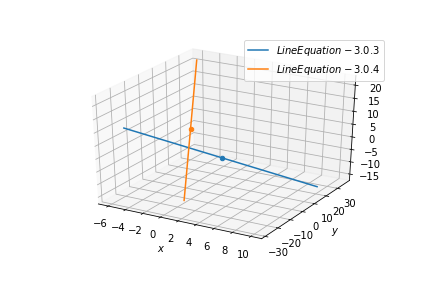
\includegraphics[width=\columnwidth]{./solutions/line_plane/74/codes/figs/Line_interest_1.png}
	\caption{Graph for equations \ref{eq:solutions/line_plane/74/codes7}}
	\label{fig:solutions/line_plane/74/codesline_equation_1}
\end{figure}


	\item 
	\begin{align}\label{eq:solutions/line_plane/74/codes12}
		\frac{x}{2} = \frac{y}{2} &= \frac{z}{1}, 
	\end{align}
	\begin{align}\label{eq:solutions/line_plane/74/codes13}
		\frac{x-5}{4} = \frac{y-2}{1} &= \frac{z-3}{8} 
	\end{align}



The above symmetric equations \ref{eq:solutions/line_plane/74/codes12}, \ref{eq:solutions/line_plane/74/codes13} can be represented in the vector form as 
\begin{align}\label{eq:solutions/line_plane/74/codes14}
	\quad \vec{r_1} &= \myvec{0\\0\\0} + \lambda_1\myvec{2\\2\\1}
	\\
	\quad \vec{r_2} &= \myvec{5\\2\\3} + \lambda_2\myvec{4\\1\\8}
\end{align}

As we have to find the angle between the vectors, we will only be taking the direction vectors into consideration. The direction vectors are $\vec{u}$ = $\myvec{2\\2\\1}$ and $\vec{v}$ = $\myvec{4\\1\\8}$. We can find the corresponding magnitude values

\begin{align}\label{eq:solutions/line_plane/74/codes16}
	\norm{\vec{u}} =\sqrt{2^{2}+2^{2}+1^{2}} =\sqrt{9}
\end{align}
\begin{align}\label{eq:solutions/line_plane/74/codes17}
	\norm{\vec{v}} =\sqrt{4^{2}+1^{2}+8^{2}} =\sqrt{81}
\end{align}

Using \ref{eq:solutions/line_plane/74/codes4}, \ref{eq:solutions/line_plane/74/codes16}, \ref{eq:solutions/line_plane/74/codes17} we get
\begin{align}
	\theta = \cos ^{-1}\frac{\myvec{2\\2\\1}^{T}\myvec{4\\1\\8}}{(\sqrt{9})(\sqrt{81})} 
	\\
	\theta = \cos ^{-1}\frac{18}{27.00}
	\\
	\theta = \cos ^{-1} (0.667)
	\\
	\theta = 48.189\degree
\end{align}

Therefore, the angle between the two lines is $48.189\degree$. See Fig. \ref{fig:solutions/line_plane/74/codesline_equation_2}


\begin{figure}
	\centering
	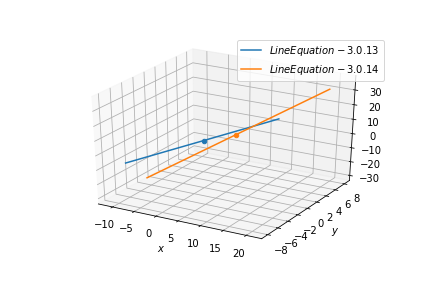
\includegraphics[width=\columnwidth]{./solutions/line_plane/74/codes/figs/Line_interest_2.png}
	\caption{Graph for equations \ref{eq:solutions/line_plane/74/codes14}}
	\label{fig:solutions/line_plane/74/codesline_equation_2}
\end{figure}
\end{enumerate}

    

\item Find a unit vector that makes an angle of $90\degree, 135\degree$ and $45\degree$ with the positive x, y and z axis respectively.
\solution 
From theory, we understand that using dot product we can find the angle between the lines 
\begin{enumerate}
	\item 
	\begin{align}\label{eq:solutions/line_plane/74/codes:5}
		\frac{x-2}{2} = \frac{y-1}{5} &= \frac{z+3}{-3}, 
	\end{align}
	\begin{align}\label{eq:solutions/line_plane/74/codes:6}
		\frac{x+2}{-1} = \frac{y-4}{8} &= \frac{z-5}{4} 
	\end{align}


The above symmetric equations \ref{eq:solutions/line_plane/74/codes:5}, \ref{eq:solutions/line_plane/74/codes:6} can be represented in the vector form as 
\begin{align}\label{eq:solutions/line_plane/74/codes7}
	\quad \vec{r_1} &= \myvec{2\\1\\-3} + \lambda_1\myvec{2\\5\\-3}
	\\
	\quad \vec{r_2} &= \myvec{-2\\4\\5} + \lambda_2\myvec{-1\\8\\4}
\end{align}

As we have to find the angle between the vectors, we will only be taking the direction vectors into consideration. The direction vectors are $\vec{u}$ = $\myvec{2\\5\\-3}$ and $\vec{v}$ = $\myvec{-1\\8\\4}$. We can find the corresponding magnitude values

\begin{align}\label{eq:solutions/line_plane/74/codes9}
	\norm{\vec{u}} =\sqrt{2^{2}+5^{2}+(-3)^{2}} =\sqrt{38}
\end{align}
\begin{align}\label{eq:solutions/line_plane/74/codes10}
	\norm{\vec{v}} =\sqrt{(-1)^{2}+8^{2}+4^{2}} =\sqrt{81}
\end{align}

Using \ref{eq:solutions/line_plane/74/codes4}, \ref{eq:solutions/line_plane/74/codes9}, \ref{eq:solutions/line_plane/74/codes10} we get
\begin{align}
	\theta = \cos ^{-1}\frac{\myvec{2\\5\\-3}^{T}\myvec{-1\\8\\4}}{(\sqrt{38})(\sqrt{81})} 
	\\
	\theta = \cos ^{-1}\frac{26}{55.4797}
	\\
	\theta = \cos ^{-1} (0.4686)
	\\
	\theta = 62.053\degree
\end{align}

Therefore, the angle between the two lines is $62.053\degree$.See Fig. \ref{fig:solutions/line_plane/74/codesline_equation_1}

\begin{figure}
	\centering
	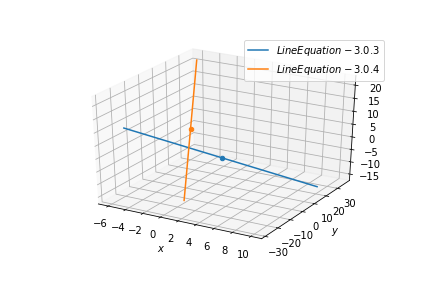
\includegraphics[width=\columnwidth]{./solutions/line_plane/74/codes/figs/Line_interest_1.png}
	\caption{Graph for equations \ref{eq:solutions/line_plane/74/codes7}}
	\label{fig:solutions/line_plane/74/codesline_equation_1}
\end{figure}


	\item 
	\begin{align}\label{eq:solutions/line_plane/74/codes12}
		\frac{x}{2} = \frac{y}{2} &= \frac{z}{1}, 
	\end{align}
	\begin{align}\label{eq:solutions/line_plane/74/codes13}
		\frac{x-5}{4} = \frac{y-2}{1} &= \frac{z-3}{8} 
	\end{align}



The above symmetric equations \ref{eq:solutions/line_plane/74/codes12}, \ref{eq:solutions/line_plane/74/codes13} can be represented in the vector form as 
\begin{align}\label{eq:solutions/line_plane/74/codes14}
	\quad \vec{r_1} &= \myvec{0\\0\\0} + \lambda_1\myvec{2\\2\\1}
	\\
	\quad \vec{r_2} &= \myvec{5\\2\\3} + \lambda_2\myvec{4\\1\\8}
\end{align}

As we have to find the angle between the vectors, we will only be taking the direction vectors into consideration. The direction vectors are $\vec{u}$ = $\myvec{2\\2\\1}$ and $\vec{v}$ = $\myvec{4\\1\\8}$. We can find the corresponding magnitude values

\begin{align}\label{eq:solutions/line_plane/74/codes16}
	\norm{\vec{u}} =\sqrt{2^{2}+2^{2}+1^{2}} =\sqrt{9}
\end{align}
\begin{align}\label{eq:solutions/line_plane/74/codes17}
	\norm{\vec{v}} =\sqrt{4^{2}+1^{2}+8^{2}} =\sqrt{81}
\end{align}

Using \ref{eq:solutions/line_plane/74/codes4}, \ref{eq:solutions/line_plane/74/codes16}, \ref{eq:solutions/line_plane/74/codes17} we get
\begin{align}
	\theta = \cos ^{-1}\frac{\myvec{2\\2\\1}^{T}\myvec{4\\1\\8}}{(\sqrt{9})(\sqrt{81})} 
	\\
	\theta = \cos ^{-1}\frac{18}{27.00}
	\\
	\theta = \cos ^{-1} (0.667)
	\\
	\theta = 48.189\degree
\end{align}

Therefore, the angle between the two lines is $48.189\degree$. See Fig. \ref{fig:solutions/line_plane/74/codesline_equation_2}


\begin{figure}
	\centering
	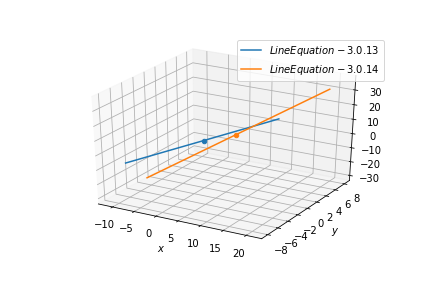
\includegraphics[width=\columnwidth]{./solutions/line_plane/74/codes/figs/Line_interest_2.png}
	\caption{Graph for equations \ref{eq:solutions/line_plane/74/codes14}}
	\label{fig:solutions/line_plane/74/codesline_equation_2}
\end{figure}
\end{enumerate}

    

\item Show that the lines with direction vectors \myvec{12\\-3\\-4}, \myvec{4\\12\\3} and \myvec{3\\-4\\12} are mutually perpendicular.
\item Show that the line through the points \myvec{1\\-1\\2}, \myvec{3\\4\\-2} is perpendicular to the line through the points   \myvec{0\\3\\2}, \myvec{3\\5\\6}.
\\
\solution 
From theory, we understand that using dot product we can find the angle between the lines 
\begin{enumerate}
	\item 
	\begin{align}\label{eq:solutions/line_plane/74/codes:5}
		\frac{x-2}{2} = \frac{y-1}{5} &= \frac{z+3}{-3}, 
	\end{align}
	\begin{align}\label{eq:solutions/line_plane/74/codes:6}
		\frac{x+2}{-1} = \frac{y-4}{8} &= \frac{z-5}{4} 
	\end{align}


The above symmetric equations \ref{eq:solutions/line_plane/74/codes:5}, \ref{eq:solutions/line_plane/74/codes:6} can be represented in the vector form as 
\begin{align}\label{eq:solutions/line_plane/74/codes7}
	\quad \vec{r_1} &= \myvec{2\\1\\-3} + \lambda_1\myvec{2\\5\\-3}
	\\
	\quad \vec{r_2} &= \myvec{-2\\4\\5} + \lambda_2\myvec{-1\\8\\4}
\end{align}

As we have to find the angle between the vectors, we will only be taking the direction vectors into consideration. The direction vectors are $\vec{u}$ = $\myvec{2\\5\\-3}$ and $\vec{v}$ = $\myvec{-1\\8\\4}$. We can find the corresponding magnitude values

\begin{align}\label{eq:solutions/line_plane/74/codes9}
	\norm{\vec{u}} =\sqrt{2^{2}+5^{2}+(-3)^{2}} =\sqrt{38}
\end{align}
\begin{align}\label{eq:solutions/line_plane/74/codes10}
	\norm{\vec{v}} =\sqrt{(-1)^{2}+8^{2}+4^{2}} =\sqrt{81}
\end{align}

Using \ref{eq:solutions/line_plane/74/codes4}, \ref{eq:solutions/line_plane/74/codes9}, \ref{eq:solutions/line_plane/74/codes10} we get
\begin{align}
	\theta = \cos ^{-1}\frac{\myvec{2\\5\\-3}^{T}\myvec{-1\\8\\4}}{(\sqrt{38})(\sqrt{81})} 
	\\
	\theta = \cos ^{-1}\frac{26}{55.4797}
	\\
	\theta = \cos ^{-1} (0.4686)
	\\
	\theta = 62.053\degree
\end{align}

Therefore, the angle between the two lines is $62.053\degree$.See Fig. \ref{fig:solutions/line_plane/74/codesline_equation_1}

\begin{figure}
	\centering
	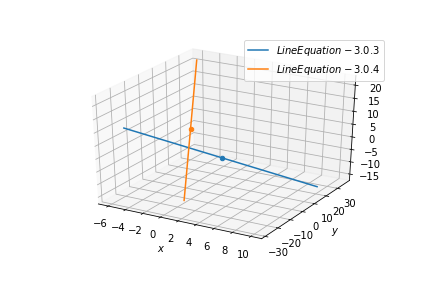
\includegraphics[width=\columnwidth]{./solutions/line_plane/74/codes/figs/Line_interest_1.png}
	\caption{Graph for equations \ref{eq:solutions/line_plane/74/codes7}}
	\label{fig:solutions/line_plane/74/codesline_equation_1}
\end{figure}


	\item 
	\begin{align}\label{eq:solutions/line_plane/74/codes12}
		\frac{x}{2} = \frac{y}{2} &= \frac{z}{1}, 
	\end{align}
	\begin{align}\label{eq:solutions/line_plane/74/codes13}
		\frac{x-5}{4} = \frac{y-2}{1} &= \frac{z-3}{8} 
	\end{align}



The above symmetric equations \ref{eq:solutions/line_plane/74/codes12}, \ref{eq:solutions/line_plane/74/codes13} can be represented in the vector form as 
\begin{align}\label{eq:solutions/line_plane/74/codes14}
	\quad \vec{r_1} &= \myvec{0\\0\\0} + \lambda_1\myvec{2\\2\\1}
	\\
	\quad \vec{r_2} &= \myvec{5\\2\\3} + \lambda_2\myvec{4\\1\\8}
\end{align}

As we have to find the angle between the vectors, we will only be taking the direction vectors into consideration. The direction vectors are $\vec{u}$ = $\myvec{2\\2\\1}$ and $\vec{v}$ = $\myvec{4\\1\\8}$. We can find the corresponding magnitude values

\begin{align}\label{eq:solutions/line_plane/74/codes16}
	\norm{\vec{u}} =\sqrt{2^{2}+2^{2}+1^{2}} =\sqrt{9}
\end{align}
\begin{align}\label{eq:solutions/line_plane/74/codes17}
	\norm{\vec{v}} =\sqrt{4^{2}+1^{2}+8^{2}} =\sqrt{81}
\end{align}

Using \ref{eq:solutions/line_plane/74/codes4}, \ref{eq:solutions/line_plane/74/codes16}, \ref{eq:solutions/line_plane/74/codes17} we get
\begin{align}
	\theta = \cos ^{-1}\frac{\myvec{2\\2\\1}^{T}\myvec{4\\1\\8}}{(\sqrt{9})(\sqrt{81})} 
	\\
	\theta = \cos ^{-1}\frac{18}{27.00}
	\\
	\theta = \cos ^{-1} (0.667)
	\\
	\theta = 48.189\degree
\end{align}

Therefore, the angle between the two lines is $48.189\degree$. See Fig. \ref{fig:solutions/line_plane/74/codesline_equation_2}


\begin{figure}
	\centering
	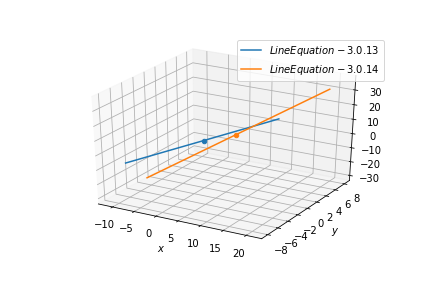
\includegraphics[width=\columnwidth]{./solutions/line_plane/74/codes/figs/Line_interest_2.png}
	\caption{Graph for equations \ref{eq:solutions/line_plane/74/codes14}}
	\label{fig:solutions/line_plane/74/codesline_equation_2}
\end{figure}
\end{enumerate}

    

\item Show that the line through the points \myvec{4\\7\\8}, \myvec{2\\3\\4} is parallel to the line through the points   \myvec{-1\\-2\\1}, \myvec{1\\2\\5}.
\\
\solution 
From theory, we understand that using dot product we can find the angle between the lines 
\begin{enumerate}
	\item 
	\begin{align}\label{eq:solutions/line_plane/74/codes:5}
		\frac{x-2}{2} = \frac{y-1}{5} &= \frac{z+3}{-3}, 
	\end{align}
	\begin{align}\label{eq:solutions/line_plane/74/codes:6}
		\frac{x+2}{-1} = \frac{y-4}{8} &= \frac{z-5}{4} 
	\end{align}


The above symmetric equations \ref{eq:solutions/line_plane/74/codes:5}, \ref{eq:solutions/line_plane/74/codes:6} can be represented in the vector form as 
\begin{align}\label{eq:solutions/line_plane/74/codes7}
	\quad \vec{r_1} &= \myvec{2\\1\\-3} + \lambda_1\myvec{2\\5\\-3}
	\\
	\quad \vec{r_2} &= \myvec{-2\\4\\5} + \lambda_2\myvec{-1\\8\\4}
\end{align}

As we have to find the angle between the vectors, we will only be taking the direction vectors into consideration. The direction vectors are $\vec{u}$ = $\myvec{2\\5\\-3}$ and $\vec{v}$ = $\myvec{-1\\8\\4}$. We can find the corresponding magnitude values

\begin{align}\label{eq:solutions/line_plane/74/codes9}
	\norm{\vec{u}} =\sqrt{2^{2}+5^{2}+(-3)^{2}} =\sqrt{38}
\end{align}
\begin{align}\label{eq:solutions/line_plane/74/codes10}
	\norm{\vec{v}} =\sqrt{(-1)^{2}+8^{2}+4^{2}} =\sqrt{81}
\end{align}

Using \ref{eq:solutions/line_plane/74/codes4}, \ref{eq:solutions/line_plane/74/codes9}, \ref{eq:solutions/line_plane/74/codes10} we get
\begin{align}
	\theta = \cos ^{-1}\frac{\myvec{2\\5\\-3}^{T}\myvec{-1\\8\\4}}{(\sqrt{38})(\sqrt{81})} 
	\\
	\theta = \cos ^{-1}\frac{26}{55.4797}
	\\
	\theta = \cos ^{-1} (0.4686)
	\\
	\theta = 62.053\degree
\end{align}

Therefore, the angle between the two lines is $62.053\degree$.See Fig. \ref{fig:solutions/line_plane/74/codesline_equation_1}

\begin{figure}
	\centering
	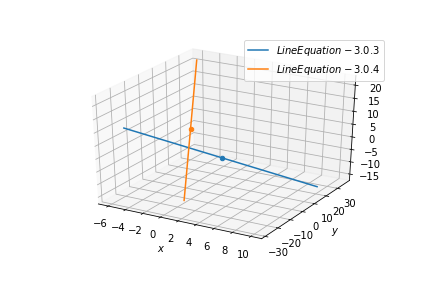
\includegraphics[width=\columnwidth]{./solutions/line_plane/74/codes/figs/Line_interest_1.png}
	\caption{Graph for equations \ref{eq:solutions/line_plane/74/codes7}}
	\label{fig:solutions/line_plane/74/codesline_equation_1}
\end{figure}


	\item 
	\begin{align}\label{eq:solutions/line_plane/74/codes12}
		\frac{x}{2} = \frac{y}{2} &= \frac{z}{1}, 
	\end{align}
	\begin{align}\label{eq:solutions/line_plane/74/codes13}
		\frac{x-5}{4} = \frac{y-2}{1} &= \frac{z-3}{8} 
	\end{align}



The above symmetric equations \ref{eq:solutions/line_plane/74/codes12}, \ref{eq:solutions/line_plane/74/codes13} can be represented in the vector form as 
\begin{align}\label{eq:solutions/line_plane/74/codes14}
	\quad \vec{r_1} &= \myvec{0\\0\\0} + \lambda_1\myvec{2\\2\\1}
	\\
	\quad \vec{r_2} &= \myvec{5\\2\\3} + \lambda_2\myvec{4\\1\\8}
\end{align}

As we have to find the angle between the vectors, we will only be taking the direction vectors into consideration. The direction vectors are $\vec{u}$ = $\myvec{2\\2\\1}$ and $\vec{v}$ = $\myvec{4\\1\\8}$. We can find the corresponding magnitude values

\begin{align}\label{eq:solutions/line_plane/74/codes16}
	\norm{\vec{u}} =\sqrt{2^{2}+2^{2}+1^{2}} =\sqrt{9}
\end{align}
\begin{align}\label{eq:solutions/line_plane/74/codes17}
	\norm{\vec{v}} =\sqrt{4^{2}+1^{2}+8^{2}} =\sqrt{81}
\end{align}

Using \ref{eq:solutions/line_plane/74/codes4}, \ref{eq:solutions/line_plane/74/codes16}, \ref{eq:solutions/line_plane/74/codes17} we get
\begin{align}
	\theta = \cos ^{-1}\frac{\myvec{2\\2\\1}^{T}\myvec{4\\1\\8}}{(\sqrt{9})(\sqrt{81})} 
	\\
	\theta = \cos ^{-1}\frac{18}{27.00}
	\\
	\theta = \cos ^{-1} (0.667)
	\\
	\theta = 48.189\degree
\end{align}

Therefore, the angle between the two lines is $48.189\degree$. See Fig. \ref{fig:solutions/line_plane/74/codesline_equation_2}


\begin{figure}
	\centering
	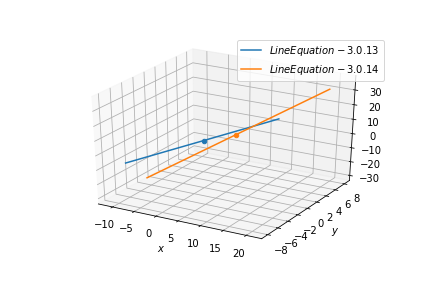
\includegraphics[width=\columnwidth]{./solutions/line_plane/74/codes/figs/Line_interest_2.png}
	\caption{Graph for equations \ref{eq:solutions/line_plane/74/codes14}}
	\label{fig:solutions/line_plane/74/codesline_equation_2}
\end{figure}
\end{enumerate}

    

\item Find a point on the x-axis, which is equidistant from the points \myvec{7\\ 6} and \myvec{3\\ 4}.
\\
\solution 
From theory, we understand that using dot product we can find the angle between the lines 
\begin{enumerate}
	\item 
	\begin{align}\label{eq:solutions/line_plane/74/codes:5}
		\frac{x-2}{2} = \frac{y-1}{5} &= \frac{z+3}{-3}, 
	\end{align}
	\begin{align}\label{eq:solutions/line_plane/74/codes:6}
		\frac{x+2}{-1} = \frac{y-4}{8} &= \frac{z-5}{4} 
	\end{align}


The above symmetric equations \ref{eq:solutions/line_plane/74/codes:5}, \ref{eq:solutions/line_plane/74/codes:6} can be represented in the vector form as 
\begin{align}\label{eq:solutions/line_plane/74/codes7}
	\quad \vec{r_1} &= \myvec{2\\1\\-3} + \lambda_1\myvec{2\\5\\-3}
	\\
	\quad \vec{r_2} &= \myvec{-2\\4\\5} + \lambda_2\myvec{-1\\8\\4}
\end{align}

As we have to find the angle between the vectors, we will only be taking the direction vectors into consideration. The direction vectors are $\vec{u}$ = $\myvec{2\\5\\-3}$ and $\vec{v}$ = $\myvec{-1\\8\\4}$. We can find the corresponding magnitude values

\begin{align}\label{eq:solutions/line_plane/74/codes9}
	\norm{\vec{u}} =\sqrt{2^{2}+5^{2}+(-3)^{2}} =\sqrt{38}
\end{align}
\begin{align}\label{eq:solutions/line_plane/74/codes10}
	\norm{\vec{v}} =\sqrt{(-1)^{2}+8^{2}+4^{2}} =\sqrt{81}
\end{align}

Using \ref{eq:solutions/line_plane/74/codes4}, \ref{eq:solutions/line_plane/74/codes9}, \ref{eq:solutions/line_plane/74/codes10} we get
\begin{align}
	\theta = \cos ^{-1}\frac{\myvec{2\\5\\-3}^{T}\myvec{-1\\8\\4}}{(\sqrt{38})(\sqrt{81})} 
	\\
	\theta = \cos ^{-1}\frac{26}{55.4797}
	\\
	\theta = \cos ^{-1} (0.4686)
	\\
	\theta = 62.053\degree
\end{align}

Therefore, the angle between the two lines is $62.053\degree$.See Fig. \ref{fig:solutions/line_plane/74/codesline_equation_1}

\begin{figure}
	\centering
	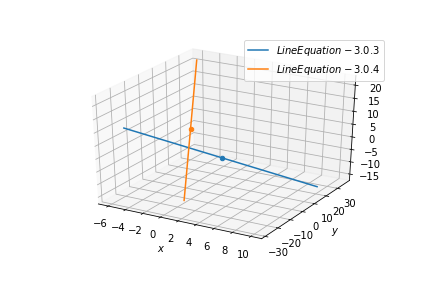
\includegraphics[width=\columnwidth]{./solutions/line_plane/74/codes/figs/Line_interest_1.png}
	\caption{Graph for equations \ref{eq:solutions/line_plane/74/codes7}}
	\label{fig:solutions/line_plane/74/codesline_equation_1}
\end{figure}


	\item 
	\begin{align}\label{eq:solutions/line_plane/74/codes12}
		\frac{x}{2} = \frac{y}{2} &= \frac{z}{1}, 
	\end{align}
	\begin{align}\label{eq:solutions/line_plane/74/codes13}
		\frac{x-5}{4} = \frac{y-2}{1} &= \frac{z-3}{8} 
	\end{align}



The above symmetric equations \ref{eq:solutions/line_plane/74/codes12}, \ref{eq:solutions/line_plane/74/codes13} can be represented in the vector form as 
\begin{align}\label{eq:solutions/line_plane/74/codes14}
	\quad \vec{r_1} &= \myvec{0\\0\\0} + \lambda_1\myvec{2\\2\\1}
	\\
	\quad \vec{r_2} &= \myvec{5\\2\\3} + \lambda_2\myvec{4\\1\\8}
\end{align}

As we have to find the angle between the vectors, we will only be taking the direction vectors into consideration. The direction vectors are $\vec{u}$ = $\myvec{2\\2\\1}$ and $\vec{v}$ = $\myvec{4\\1\\8}$. We can find the corresponding magnitude values

\begin{align}\label{eq:solutions/line_plane/74/codes16}
	\norm{\vec{u}} =\sqrt{2^{2}+2^{2}+1^{2}} =\sqrt{9}
\end{align}
\begin{align}\label{eq:solutions/line_plane/74/codes17}
	\norm{\vec{v}} =\sqrt{4^{2}+1^{2}+8^{2}} =\sqrt{81}
\end{align}

Using \ref{eq:solutions/line_plane/74/codes4}, \ref{eq:solutions/line_plane/74/codes16}, \ref{eq:solutions/line_plane/74/codes17} we get
\begin{align}
	\theta = \cos ^{-1}\frac{\myvec{2\\2\\1}^{T}\myvec{4\\1\\8}}{(\sqrt{9})(\sqrt{81})} 
	\\
	\theta = \cos ^{-1}\frac{18}{27.00}
	\\
	\theta = \cos ^{-1} (0.667)
	\\
	\theta = 48.189\degree
\end{align}

Therefore, the angle between the two lines is $48.189\degree$. See Fig. \ref{fig:solutions/line_plane/74/codesline_equation_2}


\begin{figure}
	\centering
	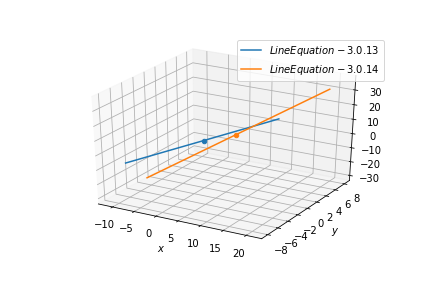
\includegraphics[width=\columnwidth]{./solutions/line_plane/74/codes/figs/Line_interest_2.png}
	\caption{Graph for equations \ref{eq:solutions/line_plane/74/codes14}}
	\label{fig:solutions/line_plane/74/codesline_equation_2}
\end{figure}
\end{enumerate}

    

\item Find the angle between the vectors 
\begin{align}
\myvec{1\\-2\\3},
\myvec{3\\-2\\1}
\end{align}
\\
\solution 
From theory, we understand that using dot product we can find the angle between the lines 
\begin{enumerate}
	\item 
	\begin{align}\label{eq:solutions/line_plane/74/codes:5}
		\frac{x-2}{2} = \frac{y-1}{5} &= \frac{z+3}{-3}, 
	\end{align}
	\begin{align}\label{eq:solutions/line_plane/74/codes:6}
		\frac{x+2}{-1} = \frac{y-4}{8} &= \frac{z-5}{4} 
	\end{align}


The above symmetric equations \ref{eq:solutions/line_plane/74/codes:5}, \ref{eq:solutions/line_plane/74/codes:6} can be represented in the vector form as 
\begin{align}\label{eq:solutions/line_plane/74/codes7}
	\quad \vec{r_1} &= \myvec{2\\1\\-3} + \lambda_1\myvec{2\\5\\-3}
	\\
	\quad \vec{r_2} &= \myvec{-2\\4\\5} + \lambda_2\myvec{-1\\8\\4}
\end{align}

As we have to find the angle between the vectors, we will only be taking the direction vectors into consideration. The direction vectors are $\vec{u}$ = $\myvec{2\\5\\-3}$ and $\vec{v}$ = $\myvec{-1\\8\\4}$. We can find the corresponding magnitude values

\begin{align}\label{eq:solutions/line_plane/74/codes9}
	\norm{\vec{u}} =\sqrt{2^{2}+5^{2}+(-3)^{2}} =\sqrt{38}
\end{align}
\begin{align}\label{eq:solutions/line_plane/74/codes10}
	\norm{\vec{v}} =\sqrt{(-1)^{2}+8^{2}+4^{2}} =\sqrt{81}
\end{align}

Using \ref{eq:solutions/line_plane/74/codes4}, \ref{eq:solutions/line_plane/74/codes9}, \ref{eq:solutions/line_plane/74/codes10} we get
\begin{align}
	\theta = \cos ^{-1}\frac{\myvec{2\\5\\-3}^{T}\myvec{-1\\8\\4}}{(\sqrt{38})(\sqrt{81})} 
	\\
	\theta = \cos ^{-1}\frac{26}{55.4797}
	\\
	\theta = \cos ^{-1} (0.4686)
	\\
	\theta = 62.053\degree
\end{align}

Therefore, the angle between the two lines is $62.053\degree$.See Fig. \ref{fig:solutions/line_plane/74/codesline_equation_1}

\begin{figure}
	\centering
	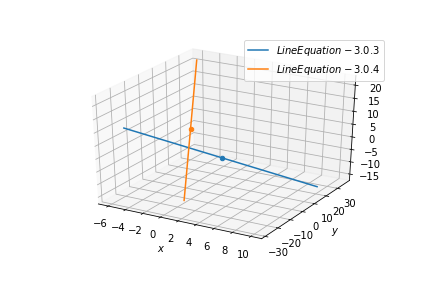
\includegraphics[width=\columnwidth]{./solutions/line_plane/74/codes/figs/Line_interest_1.png}
	\caption{Graph for equations \ref{eq:solutions/line_plane/74/codes7}}
	\label{fig:solutions/line_plane/74/codesline_equation_1}
\end{figure}


	\item 
	\begin{align}\label{eq:solutions/line_plane/74/codes12}
		\frac{x}{2} = \frac{y}{2} &= \frac{z}{1}, 
	\end{align}
	\begin{align}\label{eq:solutions/line_plane/74/codes13}
		\frac{x-5}{4} = \frac{y-2}{1} &= \frac{z-3}{8} 
	\end{align}



The above symmetric equations \ref{eq:solutions/line_plane/74/codes12}, \ref{eq:solutions/line_plane/74/codes13} can be represented in the vector form as 
\begin{align}\label{eq:solutions/line_plane/74/codes14}
	\quad \vec{r_1} &= \myvec{0\\0\\0} + \lambda_1\myvec{2\\2\\1}
	\\
	\quad \vec{r_2} &= \myvec{5\\2\\3} + \lambda_2\myvec{4\\1\\8}
\end{align}

As we have to find the angle between the vectors, we will only be taking the direction vectors into consideration. The direction vectors are $\vec{u}$ = $\myvec{2\\2\\1}$ and $\vec{v}$ = $\myvec{4\\1\\8}$. We can find the corresponding magnitude values

\begin{align}\label{eq:solutions/line_plane/74/codes16}
	\norm{\vec{u}} =\sqrt{2^{2}+2^{2}+1^{2}} =\sqrt{9}
\end{align}
\begin{align}\label{eq:solutions/line_plane/74/codes17}
	\norm{\vec{v}} =\sqrt{4^{2}+1^{2}+8^{2}} =\sqrt{81}
\end{align}

Using \ref{eq:solutions/line_plane/74/codes4}, \ref{eq:solutions/line_plane/74/codes16}, \ref{eq:solutions/line_plane/74/codes17} we get
\begin{align}
	\theta = \cos ^{-1}\frac{\myvec{2\\2\\1}^{T}\myvec{4\\1\\8}}{(\sqrt{9})(\sqrt{81})} 
	\\
	\theta = \cos ^{-1}\frac{18}{27.00}
	\\
	\theta = \cos ^{-1} (0.667)
	\\
	\theta = 48.189\degree
\end{align}

Therefore, the angle between the two lines is $48.189\degree$. See Fig. \ref{fig:solutions/line_plane/74/codesline_equation_2}


\begin{figure}
	\centering
	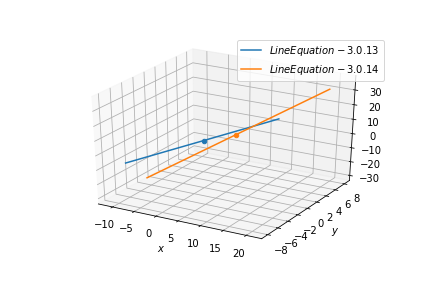
\includegraphics[width=\columnwidth]{./solutions/line_plane/74/codes/figs/Line_interest_2.png}
	\caption{Graph for equations \ref{eq:solutions/line_plane/74/codes14}}
	\label{fig:solutions/line_plane/74/codesline_equation_2}
\end{figure}
\end{enumerate}

    


\item Find the projection of the vector 
\begin{align}
\myvec{1\\3\\7}
\end{align}
on the vector
\begin{align}
\myvec{7\\-1\\8}
\end{align}
\\
\solution 
From theory, we understand that using dot product we can find the angle between the lines 
\begin{enumerate}
	\item 
	\begin{align}\label{eq:solutions/line_plane/74/codes:5}
		\frac{x-2}{2} = \frac{y-1}{5} &= \frac{z+3}{-3}, 
	\end{align}
	\begin{align}\label{eq:solutions/line_plane/74/codes:6}
		\frac{x+2}{-1} = \frac{y-4}{8} &= \frac{z-5}{4} 
	\end{align}


The above symmetric equations \ref{eq:solutions/line_plane/74/codes:5}, \ref{eq:solutions/line_plane/74/codes:6} can be represented in the vector form as 
\begin{align}\label{eq:solutions/line_plane/74/codes7}
	\quad \vec{r_1} &= \myvec{2\\1\\-3} + \lambda_1\myvec{2\\5\\-3}
	\\
	\quad \vec{r_2} &= \myvec{-2\\4\\5} + \lambda_2\myvec{-1\\8\\4}
\end{align}

As we have to find the angle between the vectors, we will only be taking the direction vectors into consideration. The direction vectors are $\vec{u}$ = $\myvec{2\\5\\-3}$ and $\vec{v}$ = $\myvec{-1\\8\\4}$. We can find the corresponding magnitude values

\begin{align}\label{eq:solutions/line_plane/74/codes9}
	\norm{\vec{u}} =\sqrt{2^{2}+5^{2}+(-3)^{2}} =\sqrt{38}
\end{align}
\begin{align}\label{eq:solutions/line_plane/74/codes10}
	\norm{\vec{v}} =\sqrt{(-1)^{2}+8^{2}+4^{2}} =\sqrt{81}
\end{align}

Using \ref{eq:solutions/line_plane/74/codes4}, \ref{eq:solutions/line_plane/74/codes9}, \ref{eq:solutions/line_plane/74/codes10} we get
\begin{align}
	\theta = \cos ^{-1}\frac{\myvec{2\\5\\-3}^{T}\myvec{-1\\8\\4}}{(\sqrt{38})(\sqrt{81})} 
	\\
	\theta = \cos ^{-1}\frac{26}{55.4797}
	\\
	\theta = \cos ^{-1} (0.4686)
	\\
	\theta = 62.053\degree
\end{align}

Therefore, the angle between the two lines is $62.053\degree$.See Fig. \ref{fig:solutions/line_plane/74/codesline_equation_1}

\begin{figure}
	\centering
	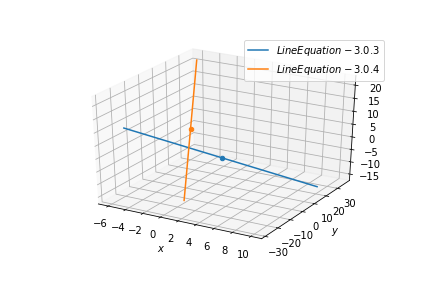
\includegraphics[width=\columnwidth]{./solutions/line_plane/74/codes/figs/Line_interest_1.png}
	\caption{Graph for equations \ref{eq:solutions/line_plane/74/codes7}}
	\label{fig:solutions/line_plane/74/codesline_equation_1}
\end{figure}


	\item 
	\begin{align}\label{eq:solutions/line_plane/74/codes12}
		\frac{x}{2} = \frac{y}{2} &= \frac{z}{1}, 
	\end{align}
	\begin{align}\label{eq:solutions/line_plane/74/codes13}
		\frac{x-5}{4} = \frac{y-2}{1} &= \frac{z-3}{8} 
	\end{align}



The above symmetric equations \ref{eq:solutions/line_plane/74/codes12}, \ref{eq:solutions/line_plane/74/codes13} can be represented in the vector form as 
\begin{align}\label{eq:solutions/line_plane/74/codes14}
	\quad \vec{r_1} &= \myvec{0\\0\\0} + \lambda_1\myvec{2\\2\\1}
	\\
	\quad \vec{r_2} &= \myvec{5\\2\\3} + \lambda_2\myvec{4\\1\\8}
\end{align}

As we have to find the angle between the vectors, we will only be taking the direction vectors into consideration. The direction vectors are $\vec{u}$ = $\myvec{2\\2\\1}$ and $\vec{v}$ = $\myvec{4\\1\\8}$. We can find the corresponding magnitude values

\begin{align}\label{eq:solutions/line_plane/74/codes16}
	\norm{\vec{u}} =\sqrt{2^{2}+2^{2}+1^{2}} =\sqrt{9}
\end{align}
\begin{align}\label{eq:solutions/line_plane/74/codes17}
	\norm{\vec{v}} =\sqrt{4^{2}+1^{2}+8^{2}} =\sqrt{81}
\end{align}

Using \ref{eq:solutions/line_plane/74/codes4}, \ref{eq:solutions/line_plane/74/codes16}, \ref{eq:solutions/line_plane/74/codes17} we get
\begin{align}
	\theta = \cos ^{-1}\frac{\myvec{2\\2\\1}^{T}\myvec{4\\1\\8}}{(\sqrt{9})(\sqrt{81})} 
	\\
	\theta = \cos ^{-1}\frac{18}{27.00}
	\\
	\theta = \cos ^{-1} (0.667)
	\\
	\theta = 48.189\degree
\end{align}

Therefore, the angle between the two lines is $48.189\degree$. See Fig. \ref{fig:solutions/line_plane/74/codesline_equation_2}


\begin{figure}
	\centering
	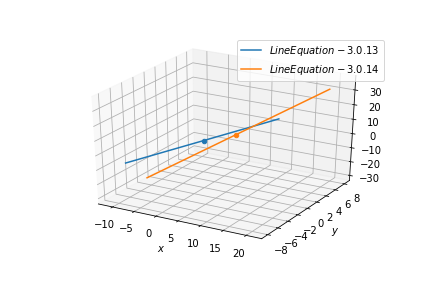
\includegraphics[width=\columnwidth]{./solutions/line_plane/74/codes/figs/Line_interest_2.png}
	\caption{Graph for equations \ref{eq:solutions/line_plane/74/codes14}}
	\label{fig:solutions/line_plane/74/codesline_equation_2}
\end{figure}
\end{enumerate}

    

\item Write down a unit vector in the xy-plane, makeing an angle of $30\degree$ with the positive direction of the x-axis.
\\
\solution 
From theory, we understand that using dot product we can find the angle between the lines 
\begin{enumerate}
	\item 
	\begin{align}\label{eq:solutions/line_plane/74/codes:5}
		\frac{x-2}{2} = \frac{y-1}{5} &= \frac{z+3}{-3}, 
	\end{align}
	\begin{align}\label{eq:solutions/line_plane/74/codes:6}
		\frac{x+2}{-1} = \frac{y-4}{8} &= \frac{z-5}{4} 
	\end{align}


The above symmetric equations \ref{eq:solutions/line_plane/74/codes:5}, \ref{eq:solutions/line_plane/74/codes:6} can be represented in the vector form as 
\begin{align}\label{eq:solutions/line_plane/74/codes7}
	\quad \vec{r_1} &= \myvec{2\\1\\-3} + \lambda_1\myvec{2\\5\\-3}
	\\
	\quad \vec{r_2} &= \myvec{-2\\4\\5} + \lambda_2\myvec{-1\\8\\4}
\end{align}

As we have to find the angle between the vectors, we will only be taking the direction vectors into consideration. The direction vectors are $\vec{u}$ = $\myvec{2\\5\\-3}$ and $\vec{v}$ = $\myvec{-1\\8\\4}$. We can find the corresponding magnitude values

\begin{align}\label{eq:solutions/line_plane/74/codes9}
	\norm{\vec{u}} =\sqrt{2^{2}+5^{2}+(-3)^{2}} =\sqrt{38}
\end{align}
\begin{align}\label{eq:solutions/line_plane/74/codes10}
	\norm{\vec{v}} =\sqrt{(-1)^{2}+8^{2}+4^{2}} =\sqrt{81}
\end{align}

Using \ref{eq:solutions/line_plane/74/codes4}, \ref{eq:solutions/line_plane/74/codes9}, \ref{eq:solutions/line_plane/74/codes10} we get
\begin{align}
	\theta = \cos ^{-1}\frac{\myvec{2\\5\\-3}^{T}\myvec{-1\\8\\4}}{(\sqrt{38})(\sqrt{81})} 
	\\
	\theta = \cos ^{-1}\frac{26}{55.4797}
	\\
	\theta = \cos ^{-1} (0.4686)
	\\
	\theta = 62.053\degree
\end{align}

Therefore, the angle between the two lines is $62.053\degree$.See Fig. \ref{fig:solutions/line_plane/74/codesline_equation_1}

\begin{figure}
	\centering
	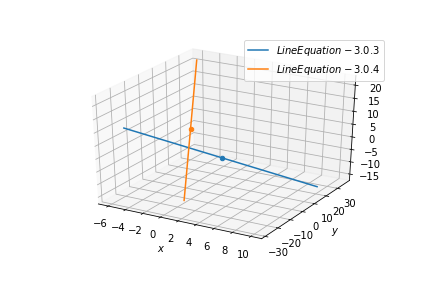
\includegraphics[width=\columnwidth]{./solutions/line_plane/74/codes/figs/Line_interest_1.png}
	\caption{Graph for equations \ref{eq:solutions/line_plane/74/codes7}}
	\label{fig:solutions/line_plane/74/codesline_equation_1}
\end{figure}


	\item 
	\begin{align}\label{eq:solutions/line_plane/74/codes12}
		\frac{x}{2} = \frac{y}{2} &= \frac{z}{1}, 
	\end{align}
	\begin{align}\label{eq:solutions/line_plane/74/codes13}
		\frac{x-5}{4} = \frac{y-2}{1} &= \frac{z-3}{8} 
	\end{align}



The above symmetric equations \ref{eq:solutions/line_plane/74/codes12}, \ref{eq:solutions/line_plane/74/codes13} can be represented in the vector form as 
\begin{align}\label{eq:solutions/line_plane/74/codes14}
	\quad \vec{r_1} &= \myvec{0\\0\\0} + \lambda_1\myvec{2\\2\\1}
	\\
	\quad \vec{r_2} &= \myvec{5\\2\\3} + \lambda_2\myvec{4\\1\\8}
\end{align}

As we have to find the angle between the vectors, we will only be taking the direction vectors into consideration. The direction vectors are $\vec{u}$ = $\myvec{2\\2\\1}$ and $\vec{v}$ = $\myvec{4\\1\\8}$. We can find the corresponding magnitude values

\begin{align}\label{eq:solutions/line_plane/74/codes16}
	\norm{\vec{u}} =\sqrt{2^{2}+2^{2}+1^{2}} =\sqrt{9}
\end{align}
\begin{align}\label{eq:solutions/line_plane/74/codes17}
	\norm{\vec{v}} =\sqrt{4^{2}+1^{2}+8^{2}} =\sqrt{81}
\end{align}

Using \ref{eq:solutions/line_plane/74/codes4}, \ref{eq:solutions/line_plane/74/codes16}, \ref{eq:solutions/line_plane/74/codes17} we get
\begin{align}
	\theta = \cos ^{-1}\frac{\myvec{2\\2\\1}^{T}\myvec{4\\1\\8}}{(\sqrt{9})(\sqrt{81})} 
	\\
	\theta = \cos ^{-1}\frac{18}{27.00}
	\\
	\theta = \cos ^{-1} (0.667)
	\\
	\theta = 48.189\degree
\end{align}

Therefore, the angle between the two lines is $48.189\degree$. See Fig. \ref{fig:solutions/line_plane/74/codesline_equation_2}


\begin{figure}
	\centering
	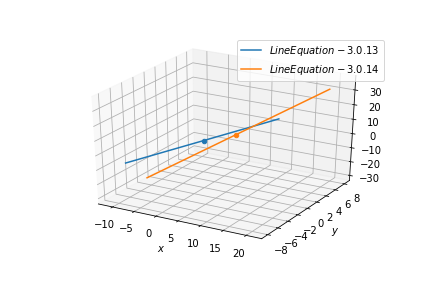
\includegraphics[width=\columnwidth]{./solutions/line_plane/74/codes/figs/Line_interest_2.png}
	\caption{Graph for equations \ref{eq:solutions/line_plane/74/codes14}}
	\label{fig:solutions/line_plane/74/codesline_equation_2}
\end{figure}
\end{enumerate}

    


\item Find the value of $x$ for which $x\myvec{1\\1\\1}$ is a unit vector.
\\
\solution
From theory, we understand that using dot product we can find the angle between the lines 
\begin{enumerate}
	\item 
	\begin{align}\label{eq:solutions/line_plane/74/codes:5}
		\frac{x-2}{2} = \frac{y-1}{5} &= \frac{z+3}{-3}, 
	\end{align}
	\begin{align}\label{eq:solutions/line_plane/74/codes:6}
		\frac{x+2}{-1} = \frac{y-4}{8} &= \frac{z-5}{4} 
	\end{align}


The above symmetric equations \ref{eq:solutions/line_plane/74/codes:5}, \ref{eq:solutions/line_plane/74/codes:6} can be represented in the vector form as 
\begin{align}\label{eq:solutions/line_plane/74/codes7}
	\quad \vec{r_1} &= \myvec{2\\1\\-3} + \lambda_1\myvec{2\\5\\-3}
	\\
	\quad \vec{r_2} &= \myvec{-2\\4\\5} + \lambda_2\myvec{-1\\8\\4}
\end{align}

As we have to find the angle between the vectors, we will only be taking the direction vectors into consideration. The direction vectors are $\vec{u}$ = $\myvec{2\\5\\-3}$ and $\vec{v}$ = $\myvec{-1\\8\\4}$. We can find the corresponding magnitude values

\begin{align}\label{eq:solutions/line_plane/74/codes9}
	\norm{\vec{u}} =\sqrt{2^{2}+5^{2}+(-3)^{2}} =\sqrt{38}
\end{align}
\begin{align}\label{eq:solutions/line_plane/74/codes10}
	\norm{\vec{v}} =\sqrt{(-1)^{2}+8^{2}+4^{2}} =\sqrt{81}
\end{align}

Using \ref{eq:solutions/line_plane/74/codes4}, \ref{eq:solutions/line_plane/74/codes9}, \ref{eq:solutions/line_plane/74/codes10} we get
\begin{align}
	\theta = \cos ^{-1}\frac{\myvec{2\\5\\-3}^{T}\myvec{-1\\8\\4}}{(\sqrt{38})(\sqrt{81})} 
	\\
	\theta = \cos ^{-1}\frac{26}{55.4797}
	\\
	\theta = \cos ^{-1} (0.4686)
	\\
	\theta = 62.053\degree
\end{align}

Therefore, the angle between the two lines is $62.053\degree$.See Fig. \ref{fig:solutions/line_plane/74/codesline_equation_1}

\begin{figure}
	\centering
	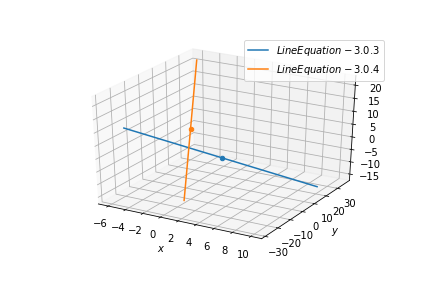
\includegraphics[width=\columnwidth]{./solutions/line_plane/74/codes/figs/Line_interest_1.png}
	\caption{Graph for equations \ref{eq:solutions/line_plane/74/codes7}}
	\label{fig:solutions/line_plane/74/codesline_equation_1}
\end{figure}


	\item 
	\begin{align}\label{eq:solutions/line_plane/74/codes12}
		\frac{x}{2} = \frac{y}{2} &= \frac{z}{1}, 
	\end{align}
	\begin{align}\label{eq:solutions/line_plane/74/codes13}
		\frac{x-5}{4} = \frac{y-2}{1} &= \frac{z-3}{8} 
	\end{align}



The above symmetric equations \ref{eq:solutions/line_plane/74/codes12}, \ref{eq:solutions/line_plane/74/codes13} can be represented in the vector form as 
\begin{align}\label{eq:solutions/line_plane/74/codes14}
	\quad \vec{r_1} &= \myvec{0\\0\\0} + \lambda_1\myvec{2\\2\\1}
	\\
	\quad \vec{r_2} &= \myvec{5\\2\\3} + \lambda_2\myvec{4\\1\\8}
\end{align}

As we have to find the angle between the vectors, we will only be taking the direction vectors into consideration. The direction vectors are $\vec{u}$ = $\myvec{2\\2\\1}$ and $\vec{v}$ = $\myvec{4\\1\\8}$. We can find the corresponding magnitude values

\begin{align}\label{eq:solutions/line_plane/74/codes16}
	\norm{\vec{u}} =\sqrt{2^{2}+2^{2}+1^{2}} =\sqrt{9}
\end{align}
\begin{align}\label{eq:solutions/line_plane/74/codes17}
	\norm{\vec{v}} =\sqrt{4^{2}+1^{2}+8^{2}} =\sqrt{81}
\end{align}

Using \ref{eq:solutions/line_plane/74/codes4}, \ref{eq:solutions/line_plane/74/codes16}, \ref{eq:solutions/line_plane/74/codes17} we get
\begin{align}
	\theta = \cos ^{-1}\frac{\myvec{2\\2\\1}^{T}\myvec{4\\1\\8}}{(\sqrt{9})(\sqrt{81})} 
	\\
	\theta = \cos ^{-1}\frac{18}{27.00}
	\\
	\theta = \cos ^{-1} (0.667)
	\\
	\theta = 48.189\degree
\end{align}

Therefore, the angle between the two lines is $48.189\degree$. See Fig. \ref{fig:solutions/line_plane/74/codesline_equation_2}


\begin{figure}
	\centering
	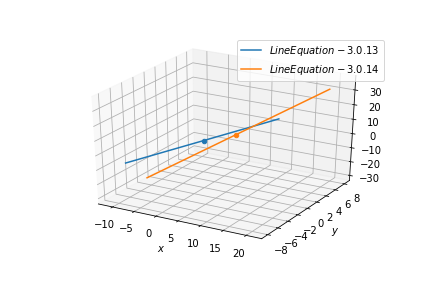
\includegraphics[width=\columnwidth]{./solutions/line_plane/74/codes/figs/Line_interest_2.png}
	\caption{Graph for equations \ref{eq:solutions/line_plane/74/codes14}}
	\label{fig:solutions/line_plane/74/codesline_equation_2}
\end{figure}
\end{enumerate}

    

\item Find the angle between the force $\vec{F} = \myvec{3\\4\\-5}$ and displacement $\vec{d} = \myvec{5\\4\\3}$.
%
\\
\solution 
From theory, we understand that using dot product we can find the angle between the lines 
\begin{enumerate}
	\item 
	\begin{align}\label{eq:solutions/line_plane/74/codes:5}
		\frac{x-2}{2} = \frac{y-1}{5} &= \frac{z+3}{-3}, 
	\end{align}
	\begin{align}\label{eq:solutions/line_plane/74/codes:6}
		\frac{x+2}{-1} = \frac{y-4}{8} &= \frac{z-5}{4} 
	\end{align}


The above symmetric equations \ref{eq:solutions/line_plane/74/codes:5}, \ref{eq:solutions/line_plane/74/codes:6} can be represented in the vector form as 
\begin{align}\label{eq:solutions/line_plane/74/codes7}
	\quad \vec{r_1} &= \myvec{2\\1\\-3} + \lambda_1\myvec{2\\5\\-3}
	\\
	\quad \vec{r_2} &= \myvec{-2\\4\\5} + \lambda_2\myvec{-1\\8\\4}
\end{align}

As we have to find the angle between the vectors, we will only be taking the direction vectors into consideration. The direction vectors are $\vec{u}$ = $\myvec{2\\5\\-3}$ and $\vec{v}$ = $\myvec{-1\\8\\4}$. We can find the corresponding magnitude values

\begin{align}\label{eq:solutions/line_plane/74/codes9}
	\norm{\vec{u}} =\sqrt{2^{2}+5^{2}+(-3)^{2}} =\sqrt{38}
\end{align}
\begin{align}\label{eq:solutions/line_plane/74/codes10}
	\norm{\vec{v}} =\sqrt{(-1)^{2}+8^{2}+4^{2}} =\sqrt{81}
\end{align}

Using \ref{eq:solutions/line_plane/74/codes4}, \ref{eq:solutions/line_plane/74/codes9}, \ref{eq:solutions/line_plane/74/codes10} we get
\begin{align}
	\theta = \cos ^{-1}\frac{\myvec{2\\5\\-3}^{T}\myvec{-1\\8\\4}}{(\sqrt{38})(\sqrt{81})} 
	\\
	\theta = \cos ^{-1}\frac{26}{55.4797}
	\\
	\theta = \cos ^{-1} (0.4686)
	\\
	\theta = 62.053\degree
\end{align}

Therefore, the angle between the two lines is $62.053\degree$.See Fig. \ref{fig:solutions/line_plane/74/codesline_equation_1}

\begin{figure}
	\centering
	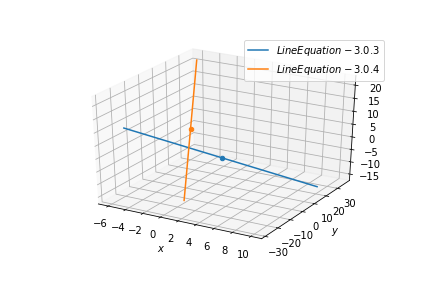
\includegraphics[width=\columnwidth]{./solutions/line_plane/74/codes/figs/Line_interest_1.png}
	\caption{Graph for equations \ref{eq:solutions/line_plane/74/codes7}}
	\label{fig:solutions/line_plane/74/codesline_equation_1}
\end{figure}


	\item 
	\begin{align}\label{eq:solutions/line_plane/74/codes12}
		\frac{x}{2} = \frac{y}{2} &= \frac{z}{1}, 
	\end{align}
	\begin{align}\label{eq:solutions/line_plane/74/codes13}
		\frac{x-5}{4} = \frac{y-2}{1} &= \frac{z-3}{8} 
	\end{align}



The above symmetric equations \ref{eq:solutions/line_plane/74/codes12}, \ref{eq:solutions/line_plane/74/codes13} can be represented in the vector form as 
\begin{align}\label{eq:solutions/line_plane/74/codes14}
	\quad \vec{r_1} &= \myvec{0\\0\\0} + \lambda_1\myvec{2\\2\\1}
	\\
	\quad \vec{r_2} &= \myvec{5\\2\\3} + \lambda_2\myvec{4\\1\\8}
\end{align}

As we have to find the angle between the vectors, we will only be taking the direction vectors into consideration. The direction vectors are $\vec{u}$ = $\myvec{2\\2\\1}$ and $\vec{v}$ = $\myvec{4\\1\\8}$. We can find the corresponding magnitude values

\begin{align}\label{eq:solutions/line_plane/74/codes16}
	\norm{\vec{u}} =\sqrt{2^{2}+2^{2}+1^{2}} =\sqrt{9}
\end{align}
\begin{align}\label{eq:solutions/line_plane/74/codes17}
	\norm{\vec{v}} =\sqrt{4^{2}+1^{2}+8^{2}} =\sqrt{81}
\end{align}

Using \ref{eq:solutions/line_plane/74/codes4}, \ref{eq:solutions/line_plane/74/codes16}, \ref{eq:solutions/line_plane/74/codes17} we get
\begin{align}
	\theta = \cos ^{-1}\frac{\myvec{2\\2\\1}^{T}\myvec{4\\1\\8}}{(\sqrt{9})(\sqrt{81})} 
	\\
	\theta = \cos ^{-1}\frac{18}{27.00}
	\\
	\theta = \cos ^{-1} (0.667)
	\\
	\theta = 48.189\degree
\end{align}

Therefore, the angle between the two lines is $48.189\degree$. See Fig. \ref{fig:solutions/line_plane/74/codesline_equation_2}


\begin{figure}
	\centering
	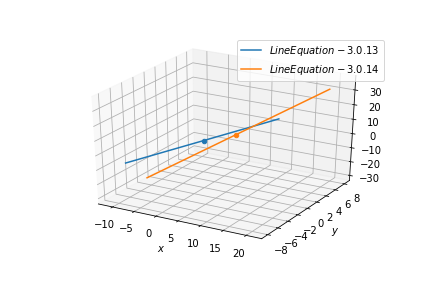
\includegraphics[width=\columnwidth]{./solutions/line_plane/74/codes/figs/Line_interest_2.png}
	\caption{Graph for equations \ref{eq:solutions/line_plane/74/codes14}}
	\label{fig:solutions/line_plane/74/codesline_equation_2}
\end{figure}
\end{enumerate}

    


\item A body constrained to move along the z-axis of a coordinate system is subject to a constant force
\begin{align}
\vec{F} = \myvec{-1\\2\\3}
\end{align}
%
What is the work done by this force in moving the body a distance of 4 m along the z-axis ?
\\
\solution 
From theory, we understand that using dot product we can find the angle between the lines 
\begin{enumerate}
	\item 
	\begin{align}\label{eq:solutions/line_plane/74/codes:5}
		\frac{x-2}{2} = \frac{y-1}{5} &= \frac{z+3}{-3}, 
	\end{align}
	\begin{align}\label{eq:solutions/line_plane/74/codes:6}
		\frac{x+2}{-1} = \frac{y-4}{8} &= \frac{z-5}{4} 
	\end{align}


The above symmetric equations \ref{eq:solutions/line_plane/74/codes:5}, \ref{eq:solutions/line_plane/74/codes:6} can be represented in the vector form as 
\begin{align}\label{eq:solutions/line_plane/74/codes7}
	\quad \vec{r_1} &= \myvec{2\\1\\-3} + \lambda_1\myvec{2\\5\\-3}
	\\
	\quad \vec{r_2} &= \myvec{-2\\4\\5} + \lambda_2\myvec{-1\\8\\4}
\end{align}

As we have to find the angle between the vectors, we will only be taking the direction vectors into consideration. The direction vectors are $\vec{u}$ = $\myvec{2\\5\\-3}$ and $\vec{v}$ = $\myvec{-1\\8\\4}$. We can find the corresponding magnitude values

\begin{align}\label{eq:solutions/line_plane/74/codes9}
	\norm{\vec{u}} =\sqrt{2^{2}+5^{2}+(-3)^{2}} =\sqrt{38}
\end{align}
\begin{align}\label{eq:solutions/line_plane/74/codes10}
	\norm{\vec{v}} =\sqrt{(-1)^{2}+8^{2}+4^{2}} =\sqrt{81}
\end{align}

Using \ref{eq:solutions/line_plane/74/codes4}, \ref{eq:solutions/line_plane/74/codes9}, \ref{eq:solutions/line_plane/74/codes10} we get
\begin{align}
	\theta = \cos ^{-1}\frac{\myvec{2\\5\\-3}^{T}\myvec{-1\\8\\4}}{(\sqrt{38})(\sqrt{81})} 
	\\
	\theta = \cos ^{-1}\frac{26}{55.4797}
	\\
	\theta = \cos ^{-1} (0.4686)
	\\
	\theta = 62.053\degree
\end{align}

Therefore, the angle between the two lines is $62.053\degree$.See Fig. \ref{fig:solutions/line_plane/74/codesline_equation_1}

\begin{figure}
	\centering
	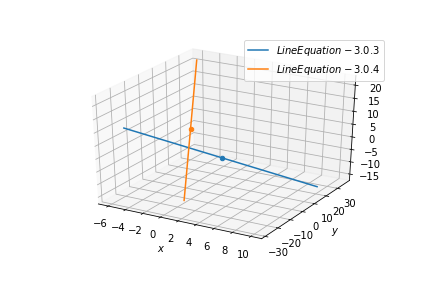
\includegraphics[width=\columnwidth]{./solutions/line_plane/74/codes/figs/Line_interest_1.png}
	\caption{Graph for equations \ref{eq:solutions/line_plane/74/codes7}}
	\label{fig:solutions/line_plane/74/codesline_equation_1}
\end{figure}


	\item 
	\begin{align}\label{eq:solutions/line_plane/74/codes12}
		\frac{x}{2} = \frac{y}{2} &= \frac{z}{1}, 
	\end{align}
	\begin{align}\label{eq:solutions/line_plane/74/codes13}
		\frac{x-5}{4} = \frac{y-2}{1} &= \frac{z-3}{8} 
	\end{align}



The above symmetric equations \ref{eq:solutions/line_plane/74/codes12}, \ref{eq:solutions/line_plane/74/codes13} can be represented in the vector form as 
\begin{align}\label{eq:solutions/line_plane/74/codes14}
	\quad \vec{r_1} &= \myvec{0\\0\\0} + \lambda_1\myvec{2\\2\\1}
	\\
	\quad \vec{r_2} &= \myvec{5\\2\\3} + \lambda_2\myvec{4\\1\\8}
\end{align}

As we have to find the angle between the vectors, we will only be taking the direction vectors into consideration. The direction vectors are $\vec{u}$ = $\myvec{2\\2\\1}$ and $\vec{v}$ = $\myvec{4\\1\\8}$. We can find the corresponding magnitude values

\begin{align}\label{eq:solutions/line_plane/74/codes16}
	\norm{\vec{u}} =\sqrt{2^{2}+2^{2}+1^{2}} =\sqrt{9}
\end{align}
\begin{align}\label{eq:solutions/line_plane/74/codes17}
	\norm{\vec{v}} =\sqrt{4^{2}+1^{2}+8^{2}} =\sqrt{81}
\end{align}

Using \ref{eq:solutions/line_plane/74/codes4}, \ref{eq:solutions/line_plane/74/codes16}, \ref{eq:solutions/line_plane/74/codes17} we get
\begin{align}
	\theta = \cos ^{-1}\frac{\myvec{2\\2\\1}^{T}\myvec{4\\1\\8}}{(\sqrt{9})(\sqrt{81})} 
	\\
	\theta = \cos ^{-1}\frac{18}{27.00}
	\\
	\theta = \cos ^{-1} (0.667)
	\\
	\theta = 48.189\degree
\end{align}

Therefore, the angle between the two lines is $48.189\degree$. See Fig. \ref{fig:solutions/line_plane/74/codesline_equation_2}


\begin{figure}
	\centering
	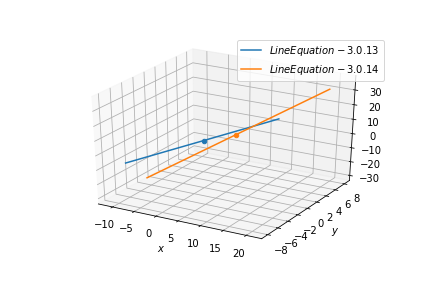
\includegraphics[width=\columnwidth]{./solutions/line_plane/74/codes/figs/Line_interest_2.png}
	\caption{Graph for equations \ref{eq:solutions/line_plane/74/codes14}}
	\label{fig:solutions/line_plane/74/codesline_equation_2}
\end{figure}
\end{enumerate}

    

\item Find the scalar and vector products of the two vectors
\begin{align}
\vec{a} = \myvec{3\\-4\\5}, 
\vec{b} = \myvec{-2\\1\\-3}
\end{align}
%
\\
\solution 
From theory, we understand that using dot product we can find the angle between the lines 
\begin{enumerate}
	\item 
	\begin{align}\label{eq:solutions/line_plane/74/codes:5}
		\frac{x-2}{2} = \frac{y-1}{5} &= \frac{z+3}{-3}, 
	\end{align}
	\begin{align}\label{eq:solutions/line_plane/74/codes:6}
		\frac{x+2}{-1} = \frac{y-4}{8} &= \frac{z-5}{4} 
	\end{align}


The above symmetric equations \ref{eq:solutions/line_plane/74/codes:5}, \ref{eq:solutions/line_plane/74/codes:6} can be represented in the vector form as 
\begin{align}\label{eq:solutions/line_plane/74/codes7}
	\quad \vec{r_1} &= \myvec{2\\1\\-3} + \lambda_1\myvec{2\\5\\-3}
	\\
	\quad \vec{r_2} &= \myvec{-2\\4\\5} + \lambda_2\myvec{-1\\8\\4}
\end{align}

As we have to find the angle between the vectors, we will only be taking the direction vectors into consideration. The direction vectors are $\vec{u}$ = $\myvec{2\\5\\-3}$ and $\vec{v}$ = $\myvec{-1\\8\\4}$. We can find the corresponding magnitude values

\begin{align}\label{eq:solutions/line_plane/74/codes9}
	\norm{\vec{u}} =\sqrt{2^{2}+5^{2}+(-3)^{2}} =\sqrt{38}
\end{align}
\begin{align}\label{eq:solutions/line_plane/74/codes10}
	\norm{\vec{v}} =\sqrt{(-1)^{2}+8^{2}+4^{2}} =\sqrt{81}
\end{align}

Using \ref{eq:solutions/line_plane/74/codes4}, \ref{eq:solutions/line_plane/74/codes9}, \ref{eq:solutions/line_plane/74/codes10} we get
\begin{align}
	\theta = \cos ^{-1}\frac{\myvec{2\\5\\-3}^{T}\myvec{-1\\8\\4}}{(\sqrt{38})(\sqrt{81})} 
	\\
	\theta = \cos ^{-1}\frac{26}{55.4797}
	\\
	\theta = \cos ^{-1} (0.4686)
	\\
	\theta = 62.053\degree
\end{align}

Therefore, the angle between the two lines is $62.053\degree$.See Fig. \ref{fig:solutions/line_plane/74/codesline_equation_1}

\begin{figure}
	\centering
	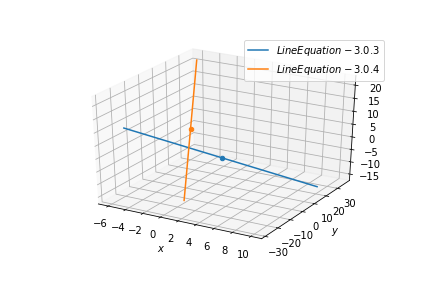
\includegraphics[width=\columnwidth]{./solutions/line_plane/74/codes/figs/Line_interest_1.png}
	\caption{Graph for equations \ref{eq:solutions/line_plane/74/codes7}}
	\label{fig:solutions/line_plane/74/codesline_equation_1}
\end{figure}


	\item 
	\begin{align}\label{eq:solutions/line_plane/74/codes12}
		\frac{x}{2} = \frac{y}{2} &= \frac{z}{1}, 
	\end{align}
	\begin{align}\label{eq:solutions/line_plane/74/codes13}
		\frac{x-5}{4} = \frac{y-2}{1} &= \frac{z-3}{8} 
	\end{align}



The above symmetric equations \ref{eq:solutions/line_plane/74/codes12}, \ref{eq:solutions/line_plane/74/codes13} can be represented in the vector form as 
\begin{align}\label{eq:solutions/line_plane/74/codes14}
	\quad \vec{r_1} &= \myvec{0\\0\\0} + \lambda_1\myvec{2\\2\\1}
	\\
	\quad \vec{r_2} &= \myvec{5\\2\\3} + \lambda_2\myvec{4\\1\\8}
\end{align}

As we have to find the angle between the vectors, we will only be taking the direction vectors into consideration. The direction vectors are $\vec{u}$ = $\myvec{2\\2\\1}$ and $\vec{v}$ = $\myvec{4\\1\\8}$. We can find the corresponding magnitude values

\begin{align}\label{eq:solutions/line_plane/74/codes16}
	\norm{\vec{u}} =\sqrt{2^{2}+2^{2}+1^{2}} =\sqrt{9}
\end{align}
\begin{align}\label{eq:solutions/line_plane/74/codes17}
	\norm{\vec{v}} =\sqrt{4^{2}+1^{2}+8^{2}} =\sqrt{81}
\end{align}

Using \ref{eq:solutions/line_plane/74/codes4}, \ref{eq:solutions/line_plane/74/codes16}, \ref{eq:solutions/line_plane/74/codes17} we get
\begin{align}
	\theta = \cos ^{-1}\frac{\myvec{2\\2\\1}^{T}\myvec{4\\1\\8}}{(\sqrt{9})(\sqrt{81})} 
	\\
	\theta = \cos ^{-1}\frac{18}{27.00}
	\\
	\theta = \cos ^{-1} (0.667)
	\\
	\theta = 48.189\degree
\end{align}

Therefore, the angle between the two lines is $48.189\degree$. See Fig. \ref{fig:solutions/line_plane/74/codesline_equation_2}


\begin{figure}
	\centering
	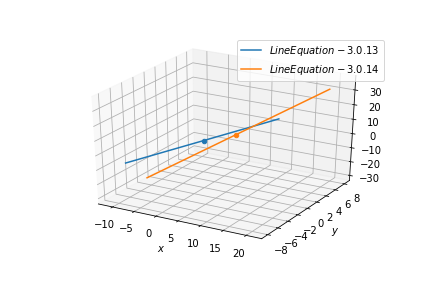
\includegraphics[width=\columnwidth]{./solutions/line_plane/74/codes/figs/Line_interest_2.png}
	\caption{Graph for equations \ref{eq:solutions/line_plane/74/codes14}}
	\label{fig:solutions/line_plane/74/codesline_equation_2}
\end{figure}
\end{enumerate}

    

\item Find the torque of a force \myvec{7\\3\\-5}
about the origin. The force
acts on a particle whose position vector is \myvec{1\\-1\\1}.
\\
\solution 
From theory, we understand that using dot product we can find the angle between the lines 
\begin{enumerate}
	\item 
	\begin{align}\label{eq:solutions/line_plane/74/codes:5}
		\frac{x-2}{2} = \frac{y-1}{5} &= \frac{z+3}{-3}, 
	\end{align}
	\begin{align}\label{eq:solutions/line_plane/74/codes:6}
		\frac{x+2}{-1} = \frac{y-4}{8} &= \frac{z-5}{4} 
	\end{align}


The above symmetric equations \ref{eq:solutions/line_plane/74/codes:5}, \ref{eq:solutions/line_plane/74/codes:6} can be represented in the vector form as 
\begin{align}\label{eq:solutions/line_plane/74/codes7}
	\quad \vec{r_1} &= \myvec{2\\1\\-3} + \lambda_1\myvec{2\\5\\-3}
	\\
	\quad \vec{r_2} &= \myvec{-2\\4\\5} + \lambda_2\myvec{-1\\8\\4}
\end{align}

As we have to find the angle between the vectors, we will only be taking the direction vectors into consideration. The direction vectors are $\vec{u}$ = $\myvec{2\\5\\-3}$ and $\vec{v}$ = $\myvec{-1\\8\\4}$. We can find the corresponding magnitude values

\begin{align}\label{eq:solutions/line_plane/74/codes9}
	\norm{\vec{u}} =\sqrt{2^{2}+5^{2}+(-3)^{2}} =\sqrt{38}
\end{align}
\begin{align}\label{eq:solutions/line_plane/74/codes10}
	\norm{\vec{v}} =\sqrt{(-1)^{2}+8^{2}+4^{2}} =\sqrt{81}
\end{align}

Using \ref{eq:solutions/line_plane/74/codes4}, \ref{eq:solutions/line_plane/74/codes9}, \ref{eq:solutions/line_plane/74/codes10} we get
\begin{align}
	\theta = \cos ^{-1}\frac{\myvec{2\\5\\-3}^{T}\myvec{-1\\8\\4}}{(\sqrt{38})(\sqrt{81})} 
	\\
	\theta = \cos ^{-1}\frac{26}{55.4797}
	\\
	\theta = \cos ^{-1} (0.4686)
	\\
	\theta = 62.053\degree
\end{align}

Therefore, the angle between the two lines is $62.053\degree$.See Fig. \ref{fig:solutions/line_plane/74/codesline_equation_1}

\begin{figure}
	\centering
	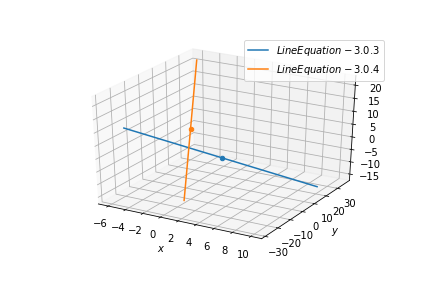
\includegraphics[width=\columnwidth]{./solutions/line_plane/74/codes/figs/Line_interest_1.png}
	\caption{Graph for equations \ref{eq:solutions/line_plane/74/codes7}}
	\label{fig:solutions/line_plane/74/codesline_equation_1}
\end{figure}


	\item 
	\begin{align}\label{eq:solutions/line_plane/74/codes12}
		\frac{x}{2} = \frac{y}{2} &= \frac{z}{1}, 
	\end{align}
	\begin{align}\label{eq:solutions/line_plane/74/codes13}
		\frac{x-5}{4} = \frac{y-2}{1} &= \frac{z-3}{8} 
	\end{align}



The above symmetric equations \ref{eq:solutions/line_plane/74/codes12}, \ref{eq:solutions/line_plane/74/codes13} can be represented in the vector form as 
\begin{align}\label{eq:solutions/line_plane/74/codes14}
	\quad \vec{r_1} &= \myvec{0\\0\\0} + \lambda_1\myvec{2\\2\\1}
	\\
	\quad \vec{r_2} &= \myvec{5\\2\\3} + \lambda_2\myvec{4\\1\\8}
\end{align}

As we have to find the angle between the vectors, we will only be taking the direction vectors into consideration. The direction vectors are $\vec{u}$ = $\myvec{2\\2\\1}$ and $\vec{v}$ = $\myvec{4\\1\\8}$. We can find the corresponding magnitude values

\begin{align}\label{eq:solutions/line_plane/74/codes16}
	\norm{\vec{u}} =\sqrt{2^{2}+2^{2}+1^{2}} =\sqrt{9}
\end{align}
\begin{align}\label{eq:solutions/line_plane/74/codes17}
	\norm{\vec{v}} =\sqrt{4^{2}+1^{2}+8^{2}} =\sqrt{81}
\end{align}

Using \ref{eq:solutions/line_plane/74/codes4}, \ref{eq:solutions/line_plane/74/codes16}, \ref{eq:solutions/line_plane/74/codes17} we get
\begin{align}
	\theta = \cos ^{-1}\frac{\myvec{2\\2\\1}^{T}\myvec{4\\1\\8}}{(\sqrt{9})(\sqrt{81})} 
	\\
	\theta = \cos ^{-1}\frac{18}{27.00}
	\\
	\theta = \cos ^{-1} (0.667)
	\\
	\theta = 48.189\degree
\end{align}

Therefore, the angle between the two lines is $48.189\degree$. See Fig. \ref{fig:solutions/line_plane/74/codesline_equation_2}


\begin{figure}
	\centering
	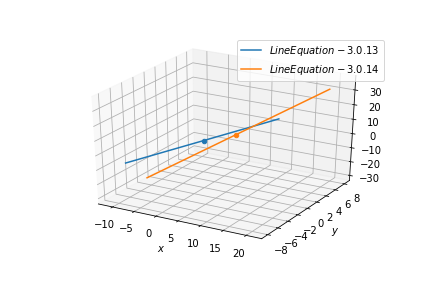
\includegraphics[width=\columnwidth]{./solutions/line_plane/74/codes/figs/Line_interest_2.png}
	\caption{Graph for equations \ref{eq:solutions/line_plane/74/codes14}}
	\label{fig:solutions/line_plane/74/codesline_equation_2}
\end{figure}
\end{enumerate}

    

%\end{enumerate}
%
